\chapter{Hardware Komponenten}\label{Komponente}

In diesem Kapitel werden die f"ur das gesamtsystem benutzten Hardware-Komponenten hinsichtlicht ihrer funktionsweise und Ansteuerung in Einzelnen erl"autert. 

\section{STM32L4 Discovery Kit}\label{LoRa}

Das STM32L4 Discovery Kit ist ein IoT Knoten, womit ein Benutzer Anwendungen mit direkter Verbindung zu einem oder mehreren Cloud-Servern entwickeln kann.
Dieses Discovery Kit erm\"oglicht eine Vielzahl von Anwendungen, indem es eine Multikink-Kommunikation (Bluetooth Low Energie) mit geringem Stromverbrauch  Multiway-Erkennung der Umwelt erm"oglicht (Siehe Abbildung \ref{Node}).

Das STM32L4 hat einen eingebetteten ST-LINK Debugger/Programmierer, eingebettete Sensoren und viele andere Features, die in dem Datenblatt \cite{B-L475E-IOT01A} erl"autert zu finden sind. Genau wegen der Vielfalt an Eingenschaften wurde dieses Board ausgew"ahlt. Man braucht kein Breadbord im Vergleich zu dem Arduino oder dem Raspberry-Pi, um die Sensoren mit den Schnittstellen (USART, SPI oder I2C) des Mikrocontrollers zu verbinden. Noch dazu eignet sich dieses Discovery Kit f"ur ein Endger"at von STMicroelectronics, da Arduino-Verbinder vorhanden sind. Dazu ist nur das Endger"at in dieser Verbinder stecken. 

\begin{figure}[h]
	\centering
	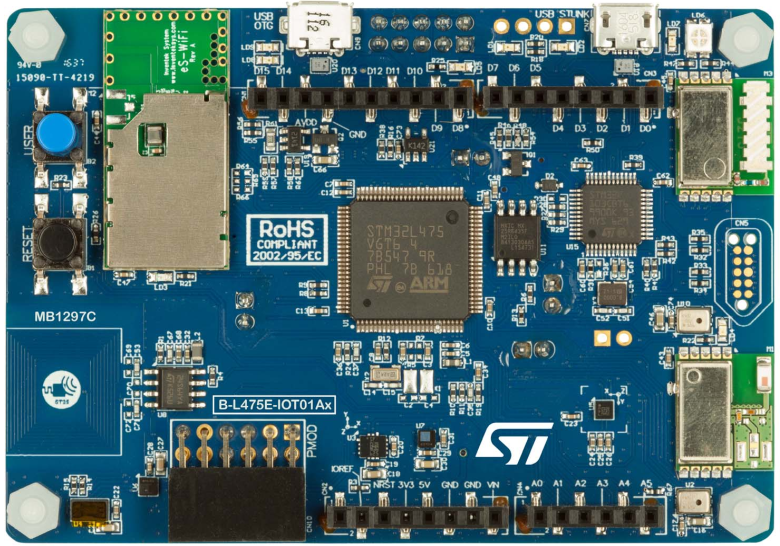
\includegraphics[width=9.5cm]{source/images/Board}
	\caption{B-L475E-IOT01A Discovery kit \cite{B-L475E-IOT01A}}\label{Node}
\end{figure}

\vspace{3cm}

F"ur diese Arbeit werden wir uns auf zwei Sensoren beschr"anken. Erstmal den HTS221\cite{HTS221} Temperatur- und Feuchtigkeitssensor und dann den LSM6DSK 3D-Gyroscope und 3D-Beschleunigungssensor \cite{LSM6DSL}. Diese Daten werden erfasst und drahtlos an den LoRaWAN-Server "ubertragen. Die folgenden Unterkapitel beschreiben, wie diese Sensoren funktionieren und erkl"aren, wie sie anzusteuern sind, damit die erhaltenen Daten im Rahmen der geforderten Toleranzen der Realit"at entsprechen. Laut dem Datenblatt ist mit einer Temperaturgenauigkeit von \textpm 0.5\textdegree{}c und einer Feuchtigkeitsgenauigkeit von \textpm 3.5\%   zu rechnen. 

\subsection {HTS221 Temperatursensor- und Feuchtigkeitssensor}\label{Temp}
In diesem Unterkapitel wird der HTS221 Temperatur- und Feuchtigkeitssensor beschrieben und erkl"art wie die Temperatur und die Feuchtigkeit zu ermitteln sind.

Der HTS221 Sensor misst die relative Feuchtigkeit(H) und die Temperatur (T) und speichert die Daten (16-Bits von Datentyp Integer) als Zweierkomplement. Diese Daten k"onnen "uber I2C- oder SPI-Schnittstelle gelesen werden. Die gespeicherte Daten sind Rohdaten, die am Ausgang von dem Analog-Digital-Converter (ADC) verf"ugbar sind (Siehe Abbildung \ref{HT_sensor}). Um die Temperatur in \textdegree{}c und die relative Feuchtigkeit in \% zu bekommen, muss man die Daten aus den Registern auslesen und mit Hilfe der Formel \ref{HumFormel} und \ref{TempFormel} die richtigen Werten herausfinden.

\begin{figure}[h]
	\centering
	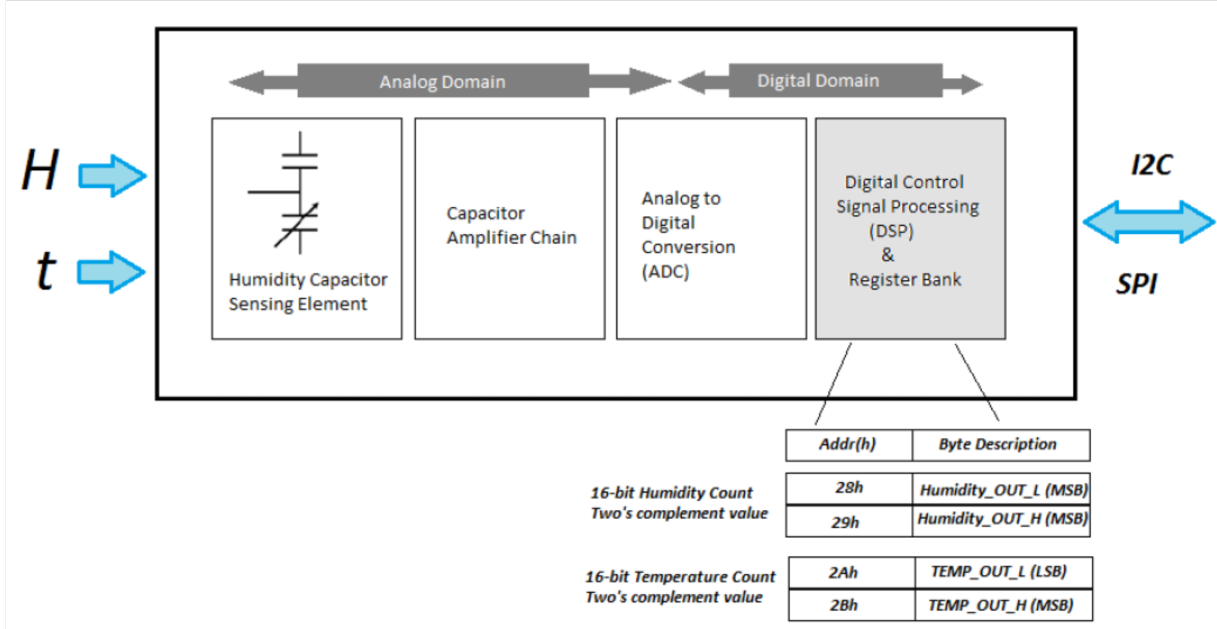
\includegraphics[width=14cm]{source/images/HTS221_sensor}
	\caption{Humidity sensor analog-to-digital flow \cite{HTS221}}\label{HT_sensor}
\end{figure}

\subsubsection{Feuchtigkeit ermitteln}

An dieser Stelle wird erkl"art wie die Feuchtigkeit von dem Sensor ermittelt wird.
Der HTS221 Sensor speichert den Feuchtigkeitswert in Rohz"alungen in zwei 8-Bit-Registern:
\begin{itemize}
	\item \textit{H\_OUT\_H} (0x29) (H"ochstwertige Bits)
	\item \textit{H\_OUT\_L} (0x28) (Niedrigswertige Bits)
\end{itemize}

Die zwei Bytes werden verkettet, um ein Zweierkomplement dargestelltes 16-Bit Wort zu bilden. Der relative Feuchtigkeitswert muss durch lineare Interpolation
der Register (\textit{HUMIDITY\_OUT\_H} \& \textit{HUMIDITY\_OUT\_L}) mit den Kalibrierregistern berechnet werden.

Der HTS221 Sensor ist bei der Herstellung schon kalibriert und die erforderlichen Koeffizienten sind ADC 16-Bit-Werte, die in den internen Register des Sensors zu lesen sind. Eine weitere Kalibrierung durch den Benutzer ist nicht erforderlich.

Die Tabelle \ref{tab:Reg_H} stellt die Register dar, in dem die Kalibrierwerte zur Ermittlung der relativen Feuchtigkeit gespeichert sind.

\begin{center}
	\begin{table}[htbp] 
		\centering 
		\Large
	%	\footnote{(u16) 16Bit-Wert ohne Vorzeichen, (s16) 16-Bit-wert mit Vorzeichen}
		\begin{tabular}{l|c|r}
			\textbf{Variable} & 	\textbf{Adresse} & \textbf{Format}\footnotemark\\
			\hline
			\textit{H0\_rH\_x2}	& 0x30	& u(8) \\
			\hline
			\textit{H1\_rH\_x2}	& 0x31	& u(8)\\
			\hline
			\textit{H0\_TO\_OUT\_H} & 0x36	& s(16)\\
			\hline
			\textit{H0\_TO\_OUT\_L} 	& 0x37  & s(16)\\
			\hline
			\textit{H1\_TO\_OUT\_H}	& 0x3A	& s(16)\\
			\hline
			\textit{H1\_TO\_OUT\_L} 	& 0x3B  & s(16)\
		\end{tabular} 
		\caption{Kalibrierregister f"ur relative Feuchtigkeit} 
		\label{tab:Reg_H} 
		 
	\end{table}
\end{center}
\footnotetext{(u8) 16Bit-Wert ohne Vorzeichen, (s16) 16Bit-Wert mit Vorzeichen}

Nun wissen wir welche Register zu lesen sind, damit die relative Feuchtigkeit mithilfe der Interpolation berechnet wird. Die folgenden Schritten m"ussen vor der Berechnung durchgef"uhrt werden:

\begin{itemize}
	\item Werte von \textit{H0\_rH\_x2} und \textit{H1\_rH\_x2} aus Registern 0x30 und 0x31 lesen 
	\item \textit{H0\_rH\_x2} und \textit{H1\_rH\_x2} durch zwei teilen
	\item Werte von \textit{H0\_TO\_OUT} aus Registern 0x36 und 0x37 lesen 
	\item Werte von \textit{H1\_TO\_OUT} aus Registern 0x3A und 0x3B lesen
	\item Rohdate von \textit{H\_T\_OUT} aus Registern 0x28 und 0x29 lesen
\end{itemize}

Nachdem diese Register gelesen wurden, kann nun die Berechnung der relative Feuchtigkeit erfolgen.

\begin{figure}[h]
	\centering
	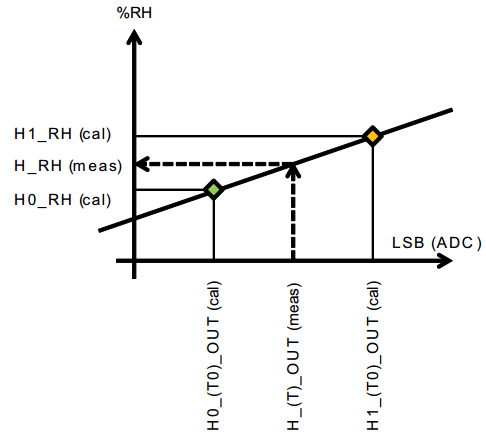
\includegraphics[width=9cm]{source/images/rH}
	\caption{Linear interpolation to convert LSB to \%RH \cite{HTS221}}\label{fig:rH}
\end{figure}

\vspace{3cm}
Aus Abbildung \ref{fig:rH} bekommt man mit Interpolation die folgende Formel \cite{HTS221}:

\begin{center}
	\[
	RH\% = \frac{((H1\_rH - H0\_rH) . (H\_T\_OUT - H0\_T0\_OUT))}{(H1\_T0\_OUT - H1\_T0\_OUT) } + H0\_rH  
	\]\label{HumFormel}
\end{center}


\subsubsection{Temperatur ermitteln}
Der HTS221 Sensor speichert die Temperaturwerten in Rohz"alungen in zwei 8-Bit-Registern:

\begin{itemize}
	\item \textit{T\_OUT\_H} (0x2A) (H"ochstwertige Bits)
	\item \textit{T\_OUT\_L} (0x2B) (Niedrigswertige Bits)
\end{itemize}

Die zwei Bytes werden verkettet, um ein Zweierkomplement dargestelltes 16-Bit Wort zu bilden. Die Polarit"at wird duch den h"ochstwertigen Bit vom \textit{T\_OUT\_H} Register bekannt gegeben.

\begin{itemize}
	\item Ist dieser Bit 0, die gelesene Temperatur ist positiv.
	\item Ist dieser Bit 1, die gelesene temperatur ist negativ. In diesem fall ist der Zweierkomplement des gesamten Wort zu bilden, um den richtigen Wert zu bekommen.
\end{itemize}

\vspace{2cm}
Auch hier ist die Temperatur durch lineare Interpolation von den Kalibrierregistern und den Registern \textit{T\_OUT\_H} und \textit{T\_OUT\_H} in Zweierkomplement zu berechnen.

Die Tabelle \ref{tab:Reg_T} stellt diese Kalibrierregister dar.

\begin{center}
	\begin{table}[htbp] 
		\centering 
		\Large
		%	\footnote{(u16) 16Bit-Wert ohne Vorzeichen, (s16) 16-Bit-wert mit Vorzeichen}
		\begin{tabular}{l|c|r}
			\textbf{Registern} & \textbf{Adresse} & \textbf{Format} \\
			\hline
			\textit{T0\_degC\_x8} & 0x32	& u(8) \\
			\hline
			\textit{T1\_degC\_x8} & 0x33	& u(8)\\
			\hline
			\textit{T1/TOmsb} & 0x35	& (u2),(u2)\\
			\hline
			\textit{T0\_OUT\_H} 	& 0x3D  & s(16)\\
			\hline
			\textit{T0\_OUT\_L} 	& 0x3C  & s(16)\\
			\hline
			\textit{T1\_OUT\_H}	& 0x3F	& s(16)\\
			\hline
			\textit{T1\_OUT\_L} 	& 0x3E  & s(16)\
		\end{tabular} 
		\caption{Kalibrierregister zur Temperaturermitllung} 
		\label{tab:Reg_T} 
		
	\end{table}
\end{center}

Da die Kalibrierregister vom Hersteller mit den korrekten Werten versehen werden, werden wir nun diese Register lesen und mithilfe der gelesenen Werten die Temperatur ermitteln. Bevor man die Temperatur mit linearer Interpolation berechnet, sind die folgenden Schritten erstmal erforderlich.

\begin{itemize}
	\item Die Koeffiziente \textit{T0\_degC\_x8} und \textit{T1\_degC\_x8} aus den Registern 0x32 und 0x33 lesen
	\item Die Werte von \textit{T0\_degC\_x8} und \textit{T1\_degC\_x8} durch 8 divisiren, um die Koeffiziente \textit{T0\_degC} und \textit{T1\_degC} zu bekommen.
	\item Die h"ochstwertige Bits von T\textit{1\_degC}(T1.9 und T1.8) und \textit{T0\_degC}(T0.9 und T0.8) aus dem Register 0x35 lesen. Diese Werte an den im Schritt 2 ermittelten Werten verketten, damit \textit{T0\_degC} und \textit{T1\_degC} vollst"andig werden.
	\item Der Wert von \textit{T0\_OUT} aus den Registern 0x3C und 0x3D lesen.
	\item Der Wert von \textit{T1\_OUT} aus den Registern 0x3E und 0x3F lesen.
	\item Der Wert von \textit{T\_OUT} aus den Registern 0x2A und 0x2B lesen.
	 	
\end{itemize}

Nachdem diese Kallibrierregister gelesen wurden, kann man mittels linearer Interpolation die Temperatur in \textdegree{}c berechnen.

\begin{figure}[h]
	\centering
	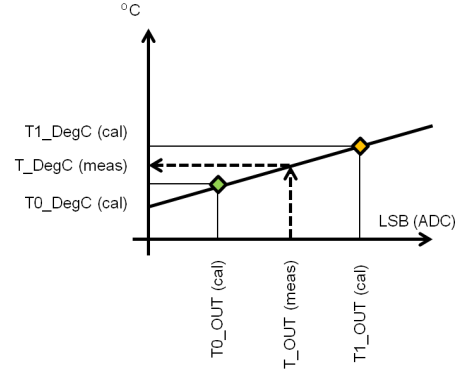
\includegraphics[width=9cm]{source/images/Temp}
	\caption{Linear interpolation to convert LSB to \textdegree{}c \cite{HTS221}}\label{fig:T}
\end{figure}

\vspace{3cm}

Abbildung \ref{gif:T} zeigt der Graph woraus die lineare Interpolation stammt. Die folgende Formel wurde sogar daraus hergeleitet.

\begin{center}
	\[
	T[\textdegree{}c] = \frac{((T1\_degC - T0\_degC) . (T\_OUT - T0\_OUT))}{(T1\_OUT - T0\_OUT) } + T0\_degC  
	\]\label{TempFormel}
\end{center}

 Da die Kalibrierwerten zur Berechnung der Temperatur und der relativen Feuchtigkeit bei der Herstellung des Bausteins vorab festgesetzt sind, soll man die Kalibrierregister bei der Programmierung nur ein mal auslesen. Dies erspart den Rechenaufwand des Mikrocontrollers.
 
\subsection{LSM6DSL 3D Gyroskope und 3D Beschleunigungssensor}\label{Acc/Gy}

Dieses Unterkapitel berichtet von dem LSM6DSL 3D-Gyroskope und 3D-Beschleuni- gungssensor. Hier ist zu entnehmen, wie die X-,Y-, und Z-Koordinaten des Sensoren zu ermitteln sind und wie der Sensor abh"angig vom Zweck skaliert werden kann.
 

Der LSM6DSL ist ein digitaler 3D-Beschleunigungsmesser und ein 3D-Gyroskopsystem mit einer digitalen seriellen I2C/SPI Schnittstelle mit einer leistung von 0.65mA im kombinierten Hochleistungsmodus.
Das Ger"at verf"ugt "uber einen von Benutzer w"ahlbaren dynamischen Beschleunigungsbereich von \textpm 2 \textbar \textpm 4 \textbar \textpm 8 \textbar \textpm 16g (g is gleich 9,81m/s) und einen Winkelgeschwindigkeitsbereich von \textpm 125 \textbar \textpm 250 \textbar \textpm 500 \textbar \textpm 1000 \textbar \textpm 2000dps (Degrees per second).
 
Das extrem geringe Gr"o\ss{}e und das geringe Gewicht des SMD-Packets machen den LSM6DSL zu einer idealen Wahl f"ur tragbare Anwendungen wie Smartphones, IoT-verbundene Ger"ate und andere Anwendungen, bei der reduzierte Paketgr"o\ss{}e und -gewicht erforderlich sind.  

Der LSM6DSL bietet drei m"ogliche Betriebskonfiguration:
\begin{itemize}
	\item nur Beschleunigungsmesser aktiv und Gyroskope inaktiv
	\item nur Gyroskope aktiv und Beschleunigungsmesser inaktiv
	\item beide aktiv mit unabh"angigem Output Data Rate (ODR) 
\end{itemize}

Der Beschleunigungsmesser und der Gyroskop k"onnen unabh"angig voneinander konfiguriert werden unteranderem: Power-down, Low-Power, Normal- und High- performance Modus. Um den Stromverbrauch des Sensors zu reduzieren, kann der Gyroskop in einem Ruhestand gesetzt werden.


Sobald das Ger"at mit Strom versorgt wird, werden die Kalibriekoeffizienten vom eingebettetem Flash-Speicher zu den internen Registers. Dieser Vorgang dauert ungef"ahr 15 milisekunden. Nach dieser Zeit fallen der Beschleunigungsmesser und der Gyroskop im Power-Down Modus. Durch der \textit{CTRL1\_XL} bzw. \textit{CTRL2\_G-}Register k"onnen die Ger"ate geweckt werben, indem man das Betriebmodus ausw"ahlt.

Wenn die Daten verf"ugbar sind, wird eine Unterbrechung (Interrupt demn"achst) ausgel"ost, wenn der entsprechende Byte vom Beschleunigungsmesser bzw. vom Gyroskop in dem \textit{INT1\_CTRL-} Register geschrieben wurde. Das vorhandensein der Daten kann nun mit Hilfe des Statusregister abgefragt werden. Das \textit{XLDA-}Bit wird auf 1 gesetzt, wenn am Ausgang des Beschleunigungsmesser ein neuer Datensatz verf"ugbar ist. Das \textit{GDS-}Bit wird suf 1 gesetzt, wenn am Gyroskopausgang ein neuer Datensatz verf"ugbar ist.

\begin{figure}[h]
	\centering
	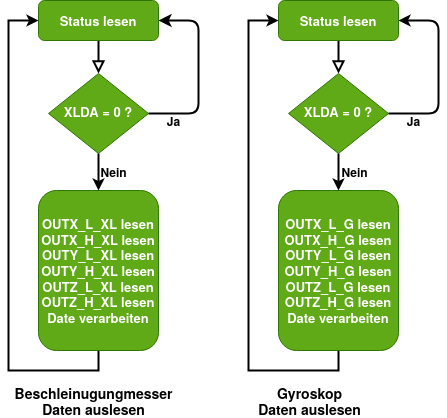
\includegraphics[width=8cm]{source/images/Gy_Acc_data}
	\caption{Flu\ss{}diagram zur Datenermitlung}\label{Gy_Acc_data}
\end{figure}

Das Abbildung \ref{Gy_Acc_data} ist der Flu\ss{}diagram zur ermitllung der Achsen- und Winkelver"anderungen des Beschleunigungsmesser und des Gyroskop.

Wie oben schon erl"autert, kann das Ger"at so eingestellet werden, dass ein neuer Satz von Messdaten durch ein Signal erkennbar wird. Das \textit{XLDA-}Bit von dem \textit{STATUS\_REG-}Register wird auf 1 gesetzt, wenn Daten aus dem Beschleunigungsmesser zum Lesen verf"ugbar sind. Das Signal kann durch den \textit{INT1-}Pin angesteuert werden, indem  das \textit{INT1\_DRDY\_XL-}Bit vom \textit{INT1\_CTRL-}Register auf 1 gestezt wird. 

F"ur den Gyroskopsensor wird das \textit{GDA-}Bit auf 1 gesetzt, wenn die Daten zum lesen verf"ugbar sind. Das Signal kann durch den \textit{INT1-}Pin angesteuert werden, indem  das \textit{INT1\_DRDY\_G-}Bit vom \textit{INT1\_CTRL-}Register auf 1 gestezt wird. Die gemessenen Beschleunigungsdaten werden in \textit{OUTX\_H\_XL-}, \textit{OUTX\_L\_XL-}, \textit{OUTY\_H\_XL-}, \textit{OUTY\_L\_-XL-}, \textit{OUTZ\_H\_XL-}, \textit{OUTZ\_L\_XL-}Register gesendet. Die gemessenen Winkelgeschwindigkeitsdaten werden dagegen in \textit{OUTX\_H\_G-}, \textit{OUTX\_L\_G-}, \textit{OUTY\_H\_G-}, \textit{OUTY\_L\_G-}, \textit{OUTZ\_H\_G-}, \textit{OUTZ\_L\_G-}Register gesendet. Die vollst"andigen Ausgangsdaten f"ur die X-,Y- und Z-Achsen sind durch die Verkettung von \textit{OUTX\_H\_XL(G)} und \textit{OUTX\_L\_-XL(G)}, \textit{OUTY\_H\_XL(G)} und \textit{OUTY\_L\_XL(G)}, \textit{OUTZ\_H\_XL(G)} und \textit{OUTZ\_L\_XL} zu erhalten, wobei die Beschleunigungsdaten und die Winkelgeschwindigkeitsdaten als 16-Bit Werte dargestellt sind.

Mit dem LSM6DSL kann man den Inhalt des unteren und oberen Teils der Ausgangsdatenregister vertauschen, sodass die Darstellung entweder Big-Endian oder Little-Endian entspricht. Dies ist m"oglich, sofern man das BLE-Bit von dem CTRL3\_C-Register auf 0 (Little-Endian Standartm"a\ss{}ig) oder auf 1 (f"ur Big-Endian) 
Big-Endian bedeutet, dass der h"ochstwertige Byte des Datensatzes in der niedrigsten Speicherstelle gespeichert wird.
Little-Endian bedeutet, dass der niedrigswertige Byte des Datensatzes in der niedrigsten Speicherstelle gespeichert wird.


Im Unterkapitel \ref{Sensoren} weden die Funktionen zur Datenermittlung in der Programmiersprache C sowohl f"ur den HTS221 (Temperatur- und Feuchtigkeitssensor) als auch f"ur den LSM6DSL (3D-Beschleunigungsensor und 3D-Gyroskop) dargestellt und erkl"art wie die Kommunicationsschnitstelle (hier I2C) zu benutzen ist.


\vspace{5cm}
\section{LoRa Endger"at: i-nucleo-lrwan1}\label{LoRa Modul}

Die im Kapitel \ref{Temp} ermittelten Sensordaten sollen laut der Aufgabestellung mit Hilfe eines drahtloses Protokol an einem Server versand werden. Um diese Daten drahtlos und auf eine lange Strecke zu "ubertragen, haben wir uns auf das LoRaWAN-Protokol entschieden. Die Gr"unde warum genau dieses Protokol ausgew"ahlt wurde, werden in diesem Kapitel genannt. Noch dazu wird nicht nur auf die Eigenschaften des benutzten Endger"at eingegangen sondern auch auf den Unterschied von diesem Modul gegen"uber anderen Modulen, die auf dem Markt zu finden sind.   
 
 
\begin{figure}[h]
	\centering
	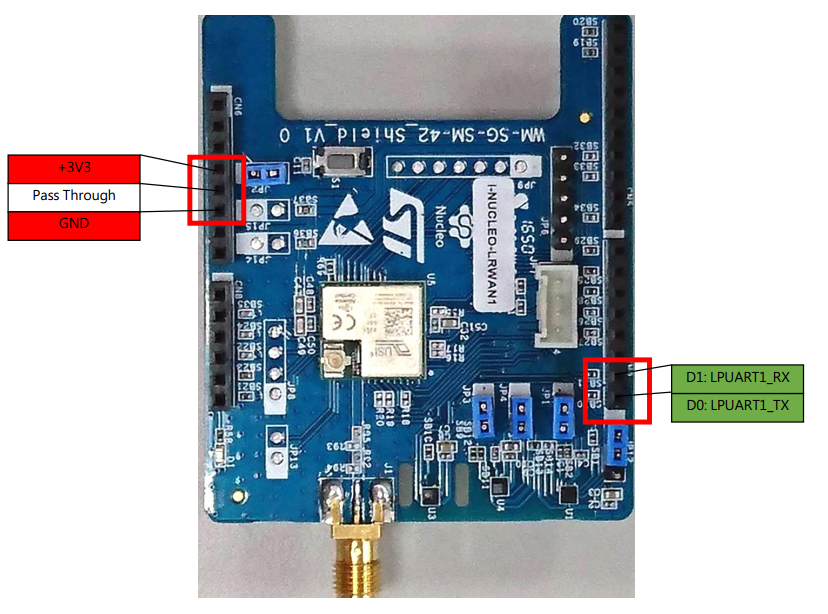
\includegraphics[width=14cm]{source/images/LoRa_mod}
	\caption{I-Nucleo-LRWAN1 \cite{LoRaMod}\label{fig:loraMod}}
\end{figure}

Abbildung \ref{fig:loraMod} zeigt das Endger"at, das zur Daten"ubertragung verwendet ist. Diese Platine mit Arduino-Connectoren und mehr ist eine integrierte L"osung, die jedem erm"oglich Anwendungen mit der LoRa-Technologie zu entwickeln. Das I-Nucleo-LRWAN1 verf"ugt "uber den USI\textregistered\ LoRaWAN\texttrademark\ Technologiemodul f"ur konsteng"unstiges und stromsparendes Weitverkehrsnetz (LPWAN), welches mit einem eingebetteten Stapel von AT-Befehle (AT-Befehl beschreiben) mitgeliefert wird.
Dieses Board wurde ausgew"ahlt, weil es durch ein externes Board wie das Nucleo-L053 oder user B-L475E-IOT01A Discovery kit \ref{Node} "uber mehrere Schnittstellen wie LPUART, SPI oder I2C angesteuert werden kann. Noch dazu verf"ugt das I-Nucleo-LRWAN1 "uber die folgenden eingebetteten Sensoren.

\begin{itemize}
	\item ST Beschleunigungs- und Magnetosensor (LSM303AGR)
	\item ST relative Feuchtigkeits- und Temperatursensor (HTS221)
	\item ST Drucksensor (LPS22HB)
\end{itemize}

Im Vergleich zu anderen Endger"aten, worauf keine Sensoren vorhanden sind, brau-cht man keine zus"atzliche Sensoren kaufen. Die Kommunikation mit einem anderen Mikrocontroller erfolgt einfach durch UART, man braucht nicht auf das integriete Radio-Modul zum Senden oder Empfangen von Daten und Befehle zu k"ummern. Das Bild \ref{fig:loraMod_intern} zeigt, dass das I-Nucleo-LRWAN1 mit einem STM32L0-Mikrocontroller versehen ist, der dazu zust"andig ist, die Kommunikation zwischen dem I-Nucleo-LRWAN1 und einem externen Mikrocontroller zu vereinfachen. Das SX1272-Chip ist das eigentliche LoRa-Radio-Modul, das die Daten oder die AT-Befehle per Funk durch die Antenne an entweder einem Gateway (Router) oder einem anderen Endger"aten sendet. 

\begin{figure}[h]
	\centering
	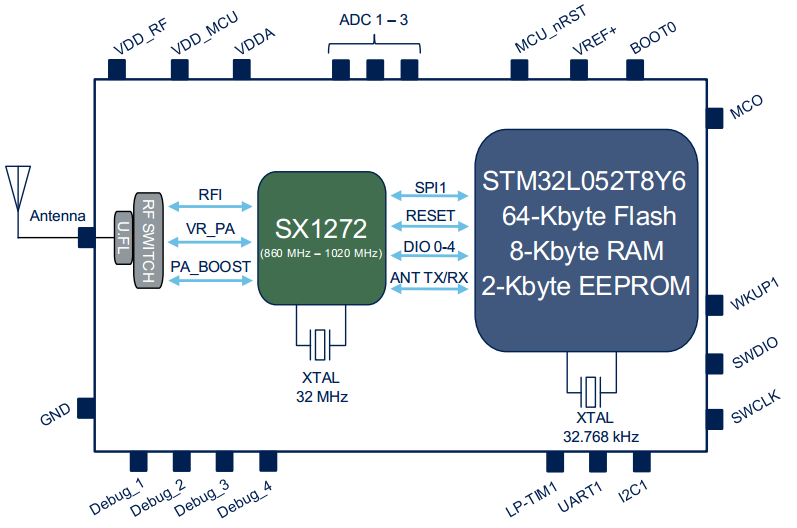
\includegraphics[width=14cm]{source/images/LoRa_Intern}
	\caption{I-Nucleo-LRWAN1 Architektur \cite{LoRaMod}\label{fig:loraMod_intern}}
\end{figure}

Das I-Nucleo-LRWAN1 wird mit Hilfe seiner Arduino-Connectoren mit einem externen Board berbunden. F"ur diese Abschlussarbeit wird dieses Endger"ats an den Arduino-Connectoren des B-L475E-IOT01A Discovery kit verbunden (Siehe Abbildung \ref{fig:loranode})

\begin{figure}[h!]
	% first include \usepackage{subfigure}
	\centering
	\subfigure[]{
		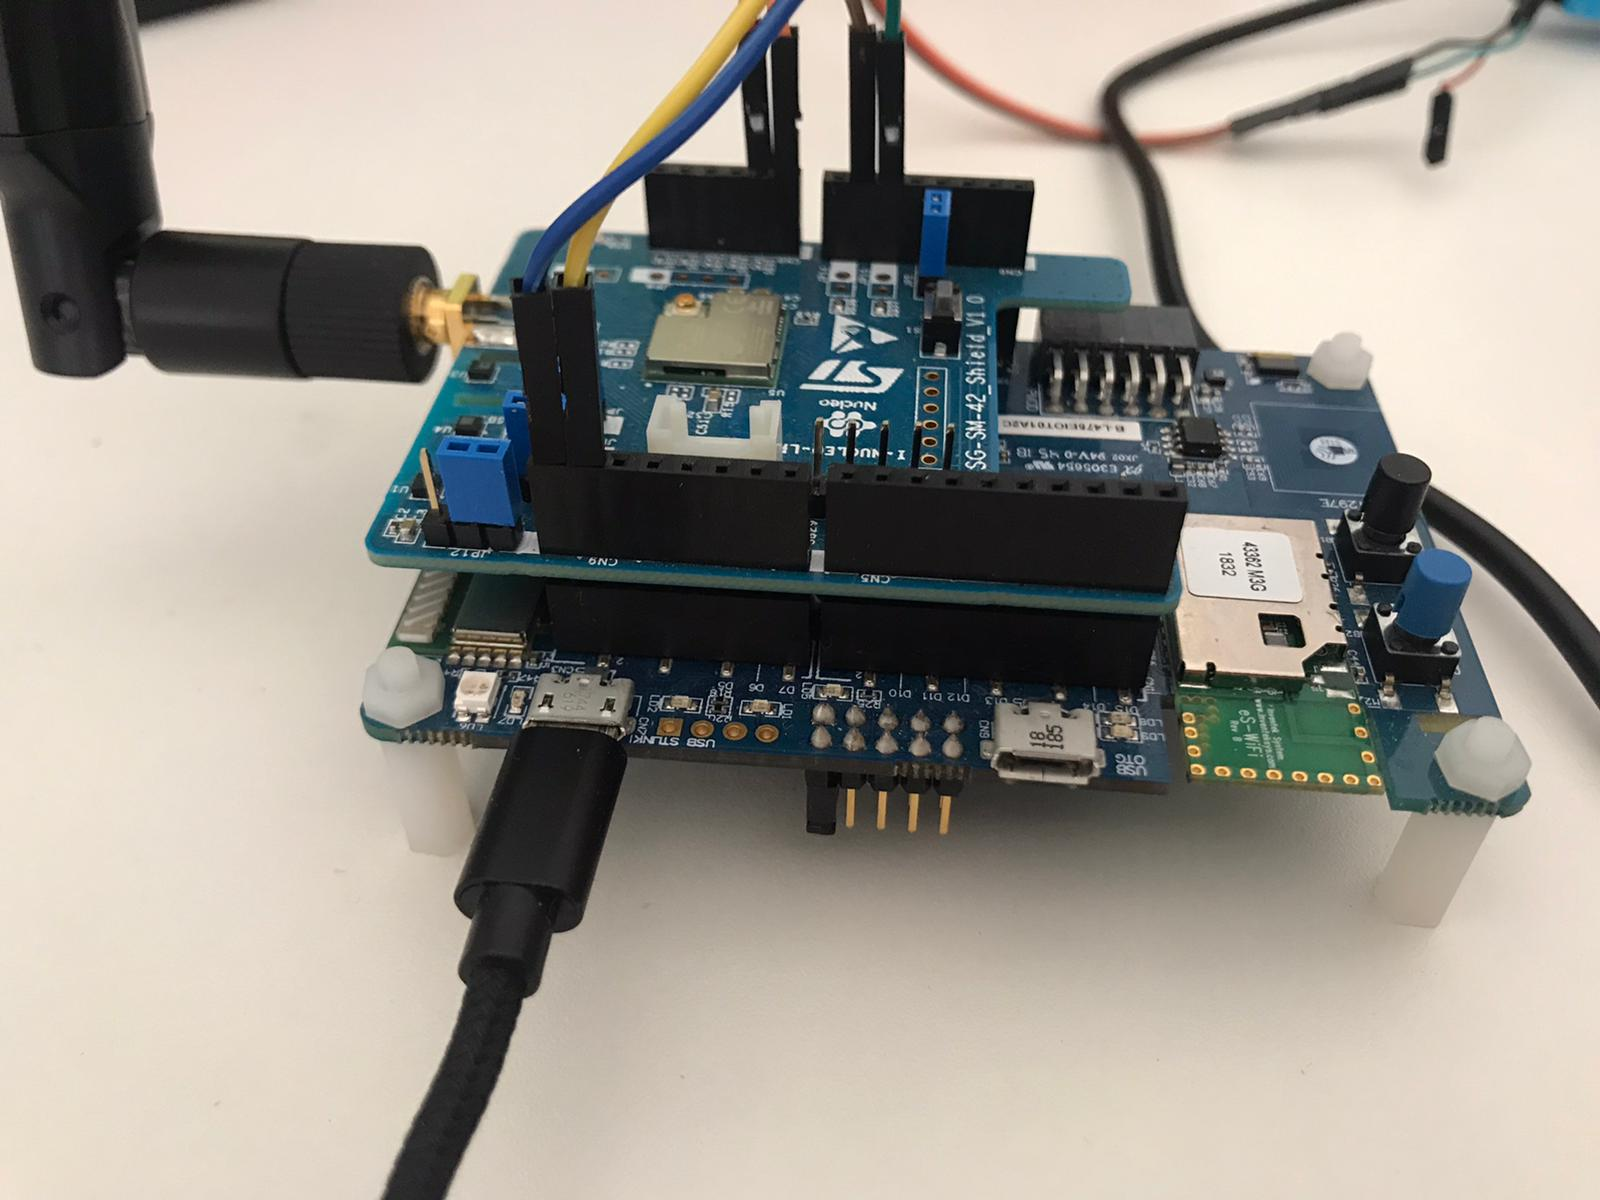
\includegraphics[ width=7cm]{source/images/Node1}
		\label{fig-subfig1}
	}
	\subfigure[]{
		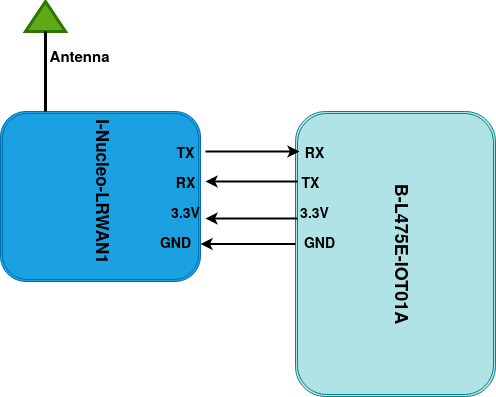
\includegraphics[width=7cm]{source/images/LABCSMARTLoRa-Node}
		\label{fig-subfig2}
	}
	\caption{LABCSMART LoRa End-Node physisches Aussehen \subref{fig-subfig1} und Verbindung \subref{fig-subfig2}\label{fig:loranode}}
\end{figure}
\vspace{10cm}
Dem Bild \ref{fig-subfig2} ist zu entnehmen, dass beide Komponnenten durch eine UART-Schnitt-stelle kommunizieren. Das I-Nucleo-LRWAN1 wird von dem  B-L475E-IOT01A mit Str-om versorgt. Die Aufgabe des B-L475E-IOT01A besteht darin, erstmal die Sensordaten zu verarbeiten, als n"achsten sendet es durch die UART-Schnittstelle AT-Befehle zur Konfiguration des I-Nucleo-LRWAN1, sodass die erhaltene Sensordaten mit Hilfe des LoRa-WAN-Protokol gesendet werden. 
\vspace{1cm}

\subsection{LoRa und LoRaWAN-Protokol}\label{LoRaWAN_P}

In diesem Teil der Thesis erfahren Sie was LoRa und das LoRaWAN-Protokol sind, als auch wie das Protokol implementiert wird, damit ein Endger"at in dem LoRaWAN-Netzwerk hinzugef"ugt wird.

\subsubsection{LoRa: Die Physikalische Schicht}

Eine einzige Technologie kann nicht alle Anwendungen des IoT decken.Technologien wie Wifi und Bluetooth Low Energie (BLE) sind wiet verbreitete Standart und decken die Kommunikation pers"onlicher Ger"ate recht gut.Die Mobilfunktechnologie passt hervorragend zur Anwendung, die einem hohen Datendurchsatz ben"otigen.

Diese Technologien sind zwar gut aber haben es bestehen einige Nachteile, wie dem hohen Energieverbrauch und die Strecke von einem Sender zu einem Empf"anger ist relativ kurz. LoRa bieten L"osungen zu diesen Nachteilen an, n"amlich eine mehrj"arige Batterielebensdauer, die "Ubertragung von kleinen Datenmengen "uber gro\ss{}e Entfernungen. LoRa ist die physikalishce Schicht oder die verwendete drahtlose Modulation, um eine lange Bereichskommunikationsverbindung zu schaffen. 

Viele "altere drahtlose Systeme verwenden die Frequenzumtastungenin (Englisch \textbf{\textit{Frequency Shifting Keying}}, Kurzform \textbf{FSK}) als physikalishce Schicht, weil es eine sehr effiziente Modulkation zur Erzielung geringer Leistung ist. LoRa basiert auf die Chirp-Spreizspektrum-Modulation (Englisch \textbf{\textit{Schirp Spread Spectrum modulation}}). Diese Modulation beha"alt die gleiche Eigenschaft der geringer Leistung wie FSK-Modulation bei und erh"oht aber deutlich die Kommunikationsreichweite. Das Chirp-Spreizspektrum wird seit Jehrzehnten auf Grund seiner Kommunikationsreichweite und seiner Robustheit gegen"uber St"orungen in der Milit"ar-und Weltraumkommunikation eingesetzt. LoRa ist derzeit die erste kosteng"unstige Implementierung f"ur dien kommerziellen Einsatz.

Es existiert konkurierende Technologien zu LoRa  wie Narrowband IoT (ND-IoT) und Sigfox. Das LoRa kann  Video- und Audio-Nachrichten nicht "ubertragen, man kann nur sehr kleine Datenpakete wie Sensordaten "ubertragen. Der Hauptpunkt von LoRa ist die Kommunikation "uber lange Strecken und die Verwendung einer sehr geringen Sendeleistung von ungef"ahr 20mW.

Die LoRa-Technologie wurde von einem kleinen franz"osischen Start-Up Namens Cycleo entwickelt. In 2012 wurde Cycleo von der Firma Semtech gekauft. Die Reichweite zwischen LoRa-Sender und -Empf"anger h"angt von der Umgebung ab, in der das Ger"at betrieben wird. Die Abdeckung von Innenr"aumen h"angt weitgehend von der Art des verwendeten Baumaterials ab. Die Tabelle \ref{tab:Range} zeigt die Reichweite der LoRa-Technologie abh"angig der Umgebung.

\begin{center}
	\begin{table}[htbp] 
		\centering 
		\Large
		\begin{tabular}{l|c|r}
			\textbf{Umgebung} & \textbf{Reichweite in kM} \\
			\hline
			St"adtische Gebiete	& 2 bis 5 \\
			\hline
			andische Gebiete & 5 bis 15\\
			\hline
			Direkte Sichtlinie	& >15 
		\end{tabular} 
		\caption{Rechweite abh"angig der Umgebung} 
		\label{tab:Range} 
		
	\end{table}
\end{center}

Es gibt aber Wirtschaftler, die dazu gekommen sind ein Weltrekord zu stellen, indem sie eine LoRa-Verbindung bis auf 200Km geschaft haben. Ein Beispiel ist Herr Andreas Spiess \cite{AndreasSpiess}.

Abbildung \ref{fig:Netz} ist zu entnehmen, dass LoRa im Vergleich zu andere Technologien wie Wifi oder 4G eine kleine Baudrate hat. Aber seine Reichweite ist deutlich gr"o\ss{}er als weit bekannte Technologien wie Bluetooth oder Wifi.


\begin{figure}[h]
	\centering
	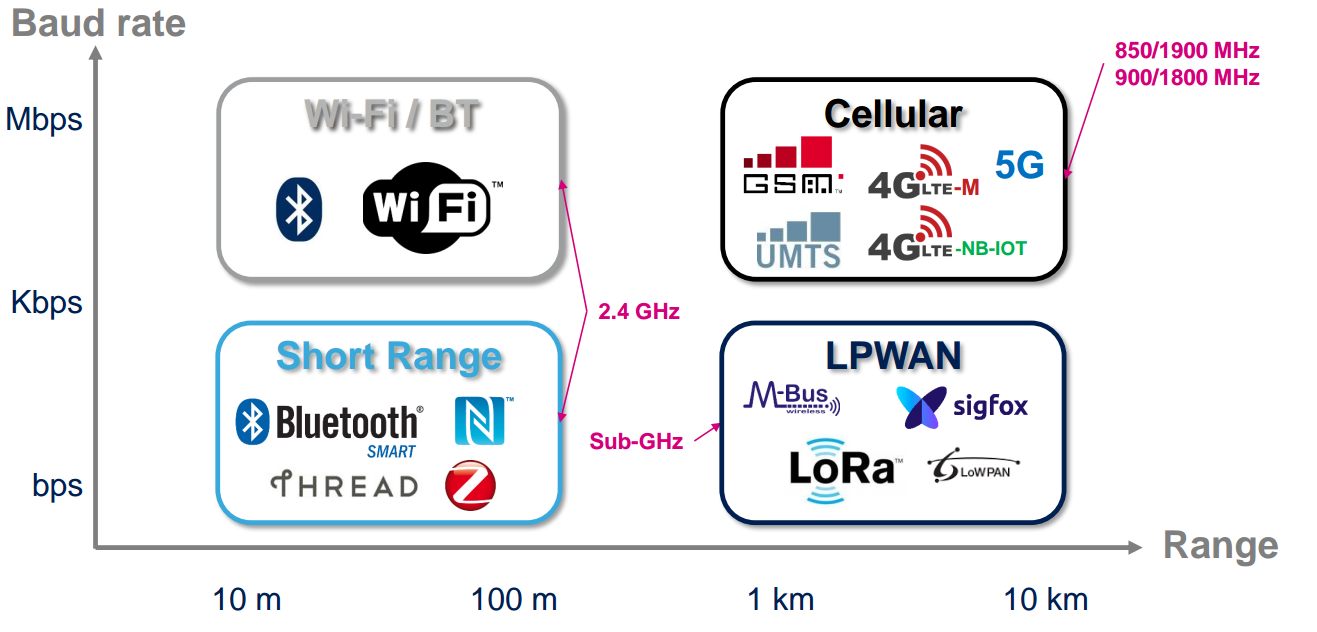
\includegraphics[width=14cm]{source/images/Communications_tech}
	\caption{Vergleich zwischen LoRa und andere IoT Kommunikationstechnologien \cite{LoRaWAN}\label{fig:Netz}}
\end{figure}

\vspace{2cm}
Die LoRa-Technologie kann man in vielen Gebiete Einsetzen. Die folgende Auflistung gibt einen groben "Uberblick auf einige Einsatzgebiete.

\begin{itemize}
	\item \textbf{Intelligente Dienstprogramme}
	\begin{itemize}
		\item "Uberwachung eines Leistungstransformators
		\item Wasserstands"uberwachung
		\item Kraftstoff"uberwachung
	\end{itemize}

	\item \textbf{Gesundheit und Hygiene}
	\begin{itemize}
		\item Temeratur- und Feuchtigkeits"uberwachung
		\item Umwelt"uberwachung
	\end{itemize}

	\item \textbf{Sicherheit}
	\begin{itemize}
		\item Radioaktivit"ats"uberwachung
		\item Intelligenter Geschwindigkeitsblitzer
	\end{itemize}

	\item \textbf{Landwirtschaft}
	\begin{itemize}
		\item "Uberwachung des Tierschutzes
		\item "Uberwachung der Pflanzenwachstumsbedingungen
	\end{itemize}

		\item \textbf{Effizienz}
	\begin{itemize}
		\item Asset Management (Tracking von Containern, Paletten)
		\item Deichmanagement (Verfolgung von Autos, Lieferwagen, Lastwagen)
	\end{itemize}
\end{itemize}

\subsubsection{LoRaWAN: Das Kommunikationsprotokoll}\label{protokol}

LoRaWAN beschreibt das Komminikationsprotokoll und die Systemarchitektur des Netzwerks, w"ahrend LoRa die physikalische Schicht, die die Fernkommunikationsverbindung erm"oglicht. Das Protokoll und die Netzwerkarchitektur haben den gr"o\ss{}en Einfulss aud die Bestimmung der Batterielebensdauer eines Endger"ats, die Netzwerkkapazit"at, die Servicequalit"at, die Sicherheit und die Vielzahl der vom Netzwerk Bereitgesellten Anwendungen. 

\begin{figure}[h]
	\centering
	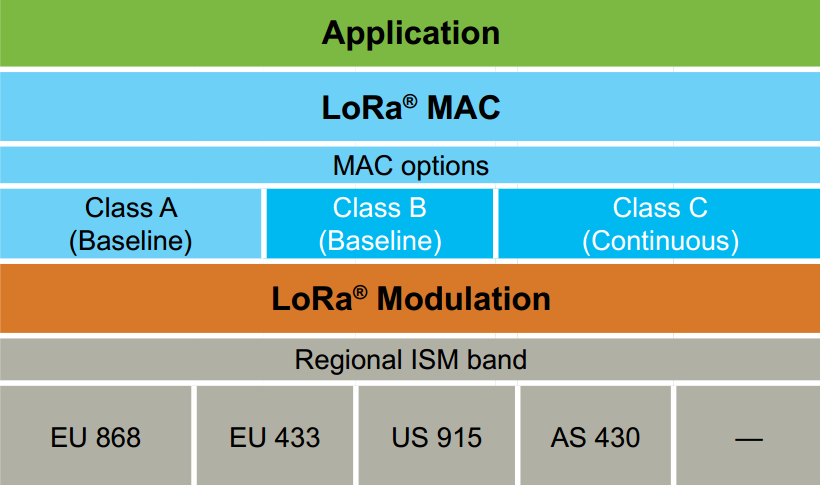
\includegraphics[width=14cm]{source/images/LoRa_MAC}
	\caption{Klassen von LoRaWAN \cite{LoRaWAN}\label{fig:LoRaMAC}}
\end{figure}

Wie es auf Abbildung \ref{fig:LoRaMAC} zu entnehmen ist, ist das LoRaWAN mit verschiedenen Schichten aufgebaut. Die erste Schicht ist die regionale Schicht, hier geht es um die Frequenzbereichen , die abh"angig von der Region zur Date"ubertragung verwendet werden k"onnen. Die ISM-Bandfrequenzen von Europa liegen zwischen 863 MHz und 870 MHz.
Als n"achstes kommt die LoRa-Modulation als physikalische Schicht des Netzwerks. LoRaWAN verf"ugt "uber viele Klassen, n"amlich die Klasse A, B und c. Diese Klassen werden sp"ater in diesem Unterkapitel im Einzelnen erkl"art. Am Ende kommt die Anwendung des LoRa-Technologie.

Alle Endger"ats funktionieren nicht gleich, dies aufgrund der von dem Entwickler implementierte Klasse.

\begin{description}
	\item [Klasse A (All end-devices) \label{classA}]: Ein Endger"at der Klasse A ermöglich eine bidirektionelle Kommunikation, wobei nach jedem Uplink eines Endger"ats f"ur kurze Zeit zwei kurzen Downlink-Empfangsfenstern folgen. Diese Empfangs fenster werden jeweils f"ur eine Zeit \textit{RECEIVE\_DELAY1}(f"ur das erste Fenster) und \textit{RECEIVE\_DELAY2} ge"offnet. Die Dauer dieser Zeiten werden sowohl in dem Endger"at als auch in dem Server gespeichert. Verglischen zu den anderen Klassen, sind Endger"ate der Klasse A die niedrigste Leistungsfresser. 
	
	Nachdem die zwei Downlink-Empfangsfenster geschlo\ss{}en sind, kann das Gateway keine weitere Downliks mehr senden. Die n"achsten Downlinks werden erst ber"ucksichtig, wenn das Endger"at ein Uplink gesendet hat.
	Das unten stehende Bild ziegt dieses Verhalten recht gut.
	
	 \begin{figure}[h]
	 	\centering
	 	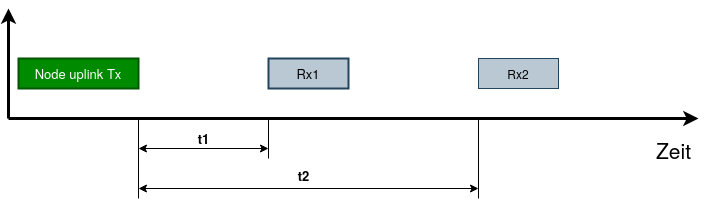
\includegraphics[width=14cm]{source/images/ClassA}
	 	\caption{Klasse A \label{fig:classA}}
	 \end{figure}
	
	\item [Klasse B (Beacon)]: Zus"atzlich zu den zuf"alligen Empf"angsfenster der Klasse A, Ger"ate der Klasse B "offnen zus"atzliche Empfangsfenster zu geplannte Zeiten. Damit das Endger"at seine Empfangsfenster an den geplannten Zeiten "offnen kann, bekommt es  ein zynchronisiertes Beacon von dem Gateway. Dies erm"oglicht dem Gateway zu wiessen, wann das Endger"at auf Downlinks wartet. Diese klasse verbraucht mehr Leistung als die Klasse A. 
	
	 \begin{figure}[h]
		\centering
		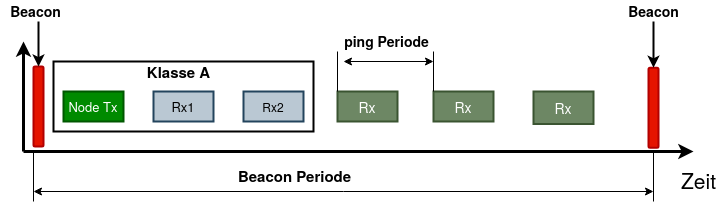
\includegraphics[width=14cm]{source/images/ClassB}
		\caption{Klasse B \label{fig:classB}}
	\end{figure}
	
	\item [Klasse C (Continuously listening)]: Endger"ate der Klasse C haben fast immer ge"offnete Empfangsfenster, die sich nur beim Senden schliessen. Diese klasse verbraucht Energie am meisten.
	
	\begin{figure}[h]
		\centering
		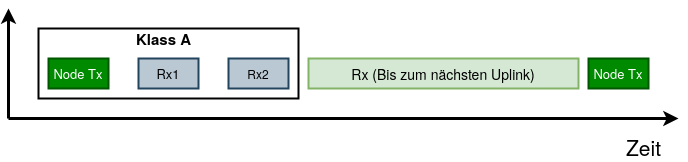
\includegraphics[width=13cm]{source/images/ClassC}
		\caption{Klasse C \label{fig:classC}}
	\end{figure}

\end{description}

\vspace{10cm}
Im Rahmen dieser Thesis wird nur die Klasse A ber"ucksichtig, weil das ausgew"ahlte Endger"at die Klasse B nicht unterst"utzt und die Klasse C zu viel Energie verbraucht. 

\subsection{Sicherung der Daten}\label{secure}

Wir wollen nicht, dass die gesendeten Informationen durch ein Dritter ohne Zugriffsrechte auf das Netzwerk die Informationen lesen kann. Unabh"angig davon, ob die Netzwerksicherheit oder die Vertraulichkeit und sicherheit der Daten gew"ahrleistet werden soll, ist das Thema sicherheit "au\ss{}erst wichtig. Eine Frage, die "ubrigens das Internet der Dinge als ganzes bettrifft.

Um die Netzwerk- und Datensicherheit zu gew"arleisten, verwendet das LoRaWAN-Netzwerk zwei AES-128-Verschl"usselung. Der erste ist der Netzwerksistzungsschl"ussel (Englisch \textbf{\textit{Network Session Key}} Kurzform \textbf{NwkSKey}) stellt die Authentizit"at der Ger"ate im Netzwerk sicher. Der zweite ist der Anwendungssitzungsschl"ussel
(Englisch \textbf{\textit{Application Session Key}} Kurzform \textbf{AppSKey}). Der NwkSkey wird von dem Endger"at und dem Server benutzt, um den Nachrichtenintegrit"atscode (Englisch \textbf{\textit{Message Integrity Code}} Kurzform \textbf{MIC}) zu berechnen und die Intergit"at aller Daten zu pr"ufen.  Es wird weiterhin verwendet, um da  Nutzdatenfeld von MAC-Daten zu verschl"usseln und zu entschl"usseln. 

Der AppSKey wird auch vom Endger"at und Server verwendet diesmal, um das Nutzdatenfeld von anwendungsspezifische Daten zu verschl"usseln und zu entschl"usseln. Die anwendungsnutzdaten werden zwischen dem Endger"at und dem Anwendungsserver Ende-zu-Ende verschl"usselt. Das hei\ss{} der Netzwerkserver kann m"oglicherweise den Inhalt der "ubertragene Daten "andern. 

\begin{figure}[h]
	\centering
	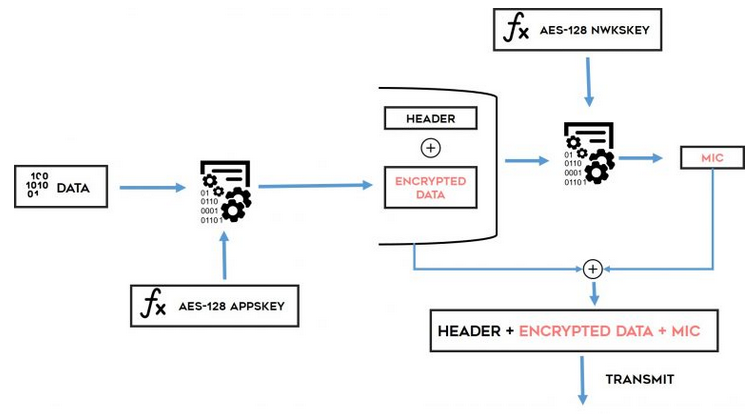
\includegraphics[width=14cm]{source/images/WAN}
	\caption{LoRaWAN-Nachricht Verschl"usselung \cite{Entcription}\label{fig:Entcription}}
\end{figure}

Laut Abblidung \ref{fig:Entcription} werden die zu sendende Daten erst mit dem AppSKey verschl"usselt. Ein Header, der andere Adressen des Endger"at enth"alt, wird an den verschl"usselten Daten hinzugef"ugt. Nach dieser Verkn"upfung wird der MIC berechnet, der nach der Berechnung an den verschl"usselten Daten und dem Header hinzugef"ugt wird. Nun k"onnen die Daten versand werden. 

Nachdem der Server die daten empfangen hat, kann die Integrit"at dieser Daten vom Server mit Hilfe des MICs gepr"uft werden. Die Daten werden nur ber"ucksichtigt, wenn der MIC stimmt, ansonsten werden sie verworven.  

\subsection{Aktivierung des Endger"ats}
Damit ein Endger"at dem LoRaWAN-Netzwerk hinzugef"ugt werden kann, muss es erst spezifiziert und aktiviert werden. Die Aktivierung eines Endger"at kann auf zwei Arten erfolgen, entweder per Over-The-Air-Aktivierung (Englisch \textbf{\textit{Over-The-Air Activation}} kurzform \textbf{OTAA}), oder per Aktivierung durch Personalisierung (Englisch \textbf{\textit{Activation By Personalization}} Kruzform \textbf{ABP}), wobei die zwei Schritte der Personalisierung und Aktivierung in einem Schritt erfolgt. 

\subsubsection{Aktivierung durch OTAA}
Damit die Over-The-Air-Aktivierung vollst"andig wird, m"ussen Endger"ate zwecks Datenaustausch mit einem Server einem Join-Verfahren folgen. Dieses Verfahren wird auch durchgef"uhrt, wenn es vorkommen w"urde, dass ein Endger"at die Sitzungsinformationen verloren hat.
Bevor ein Endger"at das Join-Verfahren startet, muss er folgende Informationen haben: Ein eine global eindeutige Endger"atekennung (\textbf{DevEUI}), eine Anwendungskennung (\textbf{AppEUI}) und ein AES-128-Schl"ussel (\textbf{AppKey}). 

\begin{description}
	\item[AppEUI:] ist 8-Byte-Wert, codiert in Hexadezimalformat und bezeichnet eine Kennung des Anwendungsanbieter.
	\item[DevEUI:] ist ein 8-Byte-Wert mit hexadezimaler Codierung und bezeichnet die eindeutige Kennung eines Endger"ats. Manche LoRa-Radiomodule beinhalten eine DevEUI vom Herstellung her. Wenn nicht schon vorhanden, diese kann vom Anwendungsanbieter gesetzt werden.
	\item[AppKey:] ist ein 16-Byte-Wert in Hexadezimalformat.Wenn ein Endge"at mit OTAA das Netzwerk beitritt, wird dieser Schl"ussel zur Herstellung des NwkSKey und des AppSKey verwendet, um die Netzwerkkommunikation und die Anwendungsdaten zu verschl"usseln und zu pr"ufen. 
\end{description}

Sobald das Endger"at mit diesen informationen versehen ist, kann es eine Join-Abfrage (\textbf{Join request}) am Server schicken. Der Server antwortet mit einem Join-Zustimmung (\textbf{Join accept}), wenn das Endger"at dem Netzwerk beitreten darf. Die Join-Accept- Nachricht wird wie ein normales Downlink gesendet aber benutzt zwei unterschiedliche Verz"ogerungen verglichen mit \textit{RECEIVE\_DELAY1} und \textit{RECEIVE\_DELAY2} der im Abschnitt \ref{classA} beschriebenen Verz"ogerungen. Diese Verz"ogerungen sind \textit{JOIN\_ACCEPT-\_DELAY1} und \textit{JOIN\_ACCEPT\_DELAY2}. Dem endger"at wird keine Antwort geschickt, wenn die Join-Abfrage abgelehnt wurde.

Die Join-Accept-Nachricht enth"alt ein 3-Byte-Anwendung Nonce (\textit{AppNonce}), eine Netzwerkkennung (\textit{NetID}), eine Endger"atadresse (\textit{DevAddr}), eine Verz"ogerung zwischen TX und RX (\textit{RxDelay}) und eine optionale Liste der Kanalfrequenz (\textit{CFList}). Die DevAddr und das AppNonce sind die wichtigste Informationen bei einer Join-Accept-Nachricht.

\begin{description}
	\item[DevAddr:] ist eine 4-Byte-Adresse, womit der Server und das Endger"at nach Aktivierung kommunizieren.   
	
	\item[AppNonce:] ist ein zuf"alliger Wert oder eine Form einer eindeutige ID, die vom Netzwekserver bereitgestellt wird und vom Endger"at verwendet, um den NwkSkey und den AppSKey abzuleiten.
	Der NwkSkey und der AppSKey werden mit der internen Funktion   \textbf{\textit{aes128\_encrypt}} (im LoRa-Radiomodule vom Hersteller zur Verf"ugung gestellt) und wird wie folgt bestimmt \cite{LoRaWAN}:
	
	\textbf{NwkSKey = aes128\_encrypt(AppKey,0x01 \textbar AppNonce \textbar NetID \textbar DevNonce \textbar pad)
	NwkSKey = aes128\_encrypt(AppKey,0x02 \textbar AppNonce \textbar NetID \textbar DevNonce \textbar pad)} 
\end{description}

Nun k"onnen Endger"ate, die dem Neztwerk beigetreten sind, Informationen mit dem Netzwerkserver austauschen (Uplinks und Downlinks). Abbildung \ref{fig:request} beschreibt das oben erl"auterte Verfahren.


\begin{figure}[h]
	\centering
	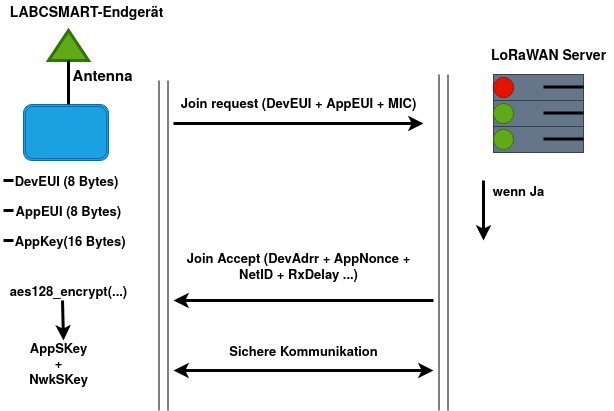
\includegraphics[width=14cm]{source/images/Join-Procedure}
	\caption{Join-Request Verfahren\label{fig:request}}
\end{figure}


\vspace{10cm}
\subsubsection{Aktivierung durch ABP}

Bei dieser Aktivierungsart, braucht das Endger"at keine Join-Abfrage senden, hier geht es um, eine direkte Bindung eines Endger"at zu einem bestimmeten Netzwerk. Das bedeutet, dass die \textit{DevAddr} und die zwei Sitzungsschl"ussel (\textit{AppSKey} und \textit{NwkSKey}) an Stelle der \textit{DevEUI}, \textit{AppEUI} und \textit{AppKey}, im Endger"at gespeichert werde. Jedes Endger"at soll einen eindetigen Satz von \textit{AppSKey} und \textit{NwkSKey}. Das Kompromittieren der Schl"ussel eines Ger"ats sollte die Sicherheit der Kommunikation anderer Ger"ate nicht beeintr"achtigen. 


Zusammengefasst ist OTAA komplexer als ABP aber bietet eine h"ohere Sicherheit. Falls ein Prototyp oder ein kleines Netzwerk erstellt werden soll, ist ABD genug. Wenn es um ein gr"o\ss{}ers Netzwerk geht, ist OTAA empfohlen, weil es sicherer und agiler ist. 

\subsection{AT Commandos}\label{AT}

Nun wissen wir was LoRa und LoRaWAN sind und wie es funktioniert, aber nicht wie Informationen (Appkey, NwkKey und mehr) dem Endger"at zugewiesen werden als auch wie die Daten am Server gesendet werden. 
Im Kapitel \ref{LoRa Modul} wurde das Wort ``AT-Befehl'' kurz erw"ahnt, in diesem Abschnitt erfahren Sie was diese Befehle sind und welche gebraucht werden, damit die eine Verbindung per OTAA oder per ABP erfolgreich wird.

Im UNIX-Systemen ist AT ein Kommando, das bewirkt, das andere Kommandos nur einmal ausgef"uhrt werden. Hier ist es benutzt, um das i-nucleo-lrwan1 einzustellen. Da das LoRa-Radiomodul sich nicht selbst einstellen kann, ist auch die Aufgabe des B-L475E-IOT01A \ref{Node} die Einstellung durchzuf"uhren. Das i-nucleo-lrwan1 verf"ugt "uber eine UART-Schnittstelle (Siehe \ref{fig:loraMod}), um mit dem B-L475E-IOT01A zu komunizieren. Diese UART-Scnittstelle hat folgende Konsolekonfiguration: 

\begin{itemize}
	\item Baudrate: 115200
	\item Daten: 8 Bit
	\item Parit"at: keine
	\item Stopbit: 1 Bit
\end{itemize}           

Die Syntax des Kommandos ist wie folgt: 
 
 \begin{itemize}
 	\item Algemeine Kommandos: 
 	\begin{itemize}
 		\item \textbf{AT:} Pr"uft ob die UART Schnittstelle benutzbar ist
 		\item \textbf{ATE [=<enable>]:}  Aktivieren oder Deaktivieren des lokalen Echos
 		\item \textbf{ATZ:} Modul zur"ucksetzen
 		\item \textbf{AT+VERB [=<enable>]:} Ausführliche Antwort aktivieren oder deaktivieren 
 	\end{itemize}
 	\item LoRa MAC-Kommandos: \textbf{AT+Kommando [=parameter]}
 	Die MAC-Kommandos werden hier nicht alle dargestellt, da es zu lang w"are sie alle zu erkl"aren. Zur Erkl"arung aller Kommandos siehe das AT-Befehlsreferenzhandbuch \cite{AT_Command}.
 	Die Zeichnen [ ] bedeuten, dass das Parameter optional ist. Mit Parametern ist ein AT-Befehl wie ein Set-Befehl, und ohne ist es ein Get-Befehl.
 \end{itemize}  

Da wir nun wiessen, wir diese Kommandos zu nutzen sind, k"onnen wir Beispiele f"ur OTAA und ABP machen (diese Einstellungen wurden getestet und funktionieren einwandfrei).

\begin{itemize}\label{LoRaconf}
	\item[\textbf{OTAA:}] Die Folgenden AT-Befehle weden von B-L475E-IOT01A nacheinander  per UART am i-nucleo-lrwan1 gesendet.
	\begin{itemize}
		\item \textbf{AT+BAND=0}: Setzt die Region des Netzwerks (Hier EU868)
		\item \textbf{AT+CLASS=0}: Die Klasse A wird verwendet 
		\item \textbf{AT+DC=1}: Deaktiviert den Auslastungsgrad 
		\item \textbf{AT+DR=0}: Setzt die TX-Datenrate (LoRa SF12/125KHz 250 Bit/s)
		\item \textbf{AT+RX2DR=0}: Setzt die TX-Datenrate (LoRa SF12/125KHz 250 Bit/s)
		\item \textbf{AT+RX1DT=1000}: Setzt die Verz"ogerung des ersten Enpfangsfenster (in ms)
		\item \textbf{AT+RX2DT=2000}: Setzt die Verz"ogerung des zweiten Enpfangsfenster (in ms)
		\item \textbf{AT+JRX1DT=5000}: Setzt die Verz"ogerung des zweiten Enpfangsfenster (in ms)
		\item \textbf{AT+JRX2DT=6000}: Setzt die Verz"ogerung des zweiten Enpfangsfenster (in ms)
		\item \textbf{AT+RF=14,8671000000,12,0,1}: Konfiguriert das LoRa-Radiomodule. Ausgansleistung: 14dBm, Frequenz: 867.1MHz, Spreading factor: SF12, Bandbreit: 125KHz, Cyclic Codingrate: 4/5.  
		\item \textbf{AT+APPEUI=ABC123ADF135CBD8}: Setzt die AppEUI
		\item \textbf{AT+AK=00112233445566778899AABBCCDDEEFF}: Setzt den AppKey 
		\item \textbf{AT+JOIN=1}: Sendet eine Join-Abfrage als OTAA
		 
	\end{itemize}
	
	\item[\textbf{ABP:}] Die Folgenden AT-Befehle weden von B-L475E-IOT01A nacheinander  per UART am i-nucleo-lrwan1 gesendet.
	\begin{itemize}
		\item \textbf{AT+BAND=0}
		\item \textbf{AT+CLASS=0} 
		\item \textbf{AT+DC=1}
		\item \textbf{AT+DR=0} 
		\item \textbf{AT+RX2DR=0}
		\item \textbf{AT+RX1DT=1000} 
		\item \textbf{AT+RX2DT=2000} 
		\item \textbf{AT+JRX1DT=5000}
		\item \textbf{AT+JRX2DT=6000} 
		\item \textbf{AT+RF=14,8671000000,12,0,1}
		\item \textbf{AT+ADDR=12345678}: Setzt die Ger"atadresse 
		\item \textbf{AT+NSK=1122334455663EAB546829CB361CAB7D}: Setzt den NwkSKey
		\item \textbf{AT+ASK=887766554433BCFACDE52476CA4598BA}: Setzt den AppSKey 
		\item \textbf{AT+JOIN=0}: Sendet eine Join-Abfrage als ABP
	\end{itemize}

	\item[\textbf{Daten senden}:] \textbf{AT+SEND=2,Daten,1}
	Hier werden die Daten durch das Port 2 gesendet. Die Daten mussen in hexadezimaler Format sein, und sollen nicht gr"o\ss{}er als 64 Bytes sein. Die 1 am Ende steht f"ur die Best"atigung des Datenempfangs. 
	
\end{itemize}

Im AT-Befehlsreferenzhabdbuch stellt das Appendix 3 Tabellen f"ur die Konfiguration der Datenrate abh"angig von der Region zur Verf"ugung.

\chapter{Gateway und LoRaWAN-Server}\label{G_S}

Nun ist es m"oglich ein Endger"at, so einzustellen, dass es f"ahig ist, Uplinks an einem LoRaWAN-Server zu senden und Downlink vom Server zu bekommen. Aber was ist das LoRaWAN-Server und wozu wird das Gateway benutzt. Diese Fragen werden in diesem Kapitel beantwortet.

\section{Gateway}\label{Gateway}

Es gibt fertige Gateways auf dem Markt, die man kaufen und direkt einsetzen kann . F"ur diese Thesis wir ein selbst gebautes Gateway benutzt. Der Grund daf"ur ist das es biliger als fertige Gateway ist, sich ein eigenes zu bauen. Noch dazu steckt eine Wissenschaftliche Idee dahinter. Zu wiessen, wie ein Gateway gebaut wird, welche Komponenten und welche Software im Spiel kommen.  

Ein Gateway ist ein Ger"at, das aus mindestens einem Konzentrator, einem Host und einer Netzverbindung zum Internet oder einen privaten Netzwerk (Ethernet, 3G, Wifi), m"oglicherweise einem GPS-Empf"anger besteht. Der Konzentrator ist ein Board, das Funkpakette senden und empfangen kann. Ein Konzentrator basiert auf einem Semtech-Mehrkanalmodem (\textbf{\textit{SX130x}}), einem Transceiver (\textbf{\textit{SX135x}}) und/oder eigenst"andige Modems mit geringem Stromverbrauch (\textbf{\textit{SX127x}}).  

Ein Host ist ein eingebetteter Computer, auf dem die Paketweiterleitung ausgef"urt wird. Der Host steuert den Konzentrator "uber eine SPI-Schnittstelle. F"ur diese Arbeit ist der Host ein Raspberry-Pi. Ein Gateway kann viele Endger"ate gleichzeitig behandeln. Die Kommunikation zwischen einem endger"at und einem Gateway ist bidirektional, das heisst das Endger"at sendet dem Gateway Daten, aber kann auch Daten von dem Gateway empfangen.

Die Kommunikation von einem Endger"at zum Gateway ist ein Uplink, w"ahrend die Kommunikation vom Gateway zum Endger"at ein Downlink ist.
Ein Endger"at sendet Uplinks als Broadcast, das heisst die gesendete Daten werden von allen Gateways des Netzwerks bekommen. Das Gateway leitet das Datenpaket an dem Netzwerkserver weiter. Der Netzwerkserver sammelt die Nachrichten aller Gateways, filtert doppelte Daten heraus und bestimmt das Gateway mit der besten Rezeption. Der Netzwerkserver leitet seine Daten zu dem entsprechenden Anwendungsserver, womit der Nutzer die Sensordaten ansehen und/oder verarbeiten kann.

Bekommt den Netzwerkserver eine Antwort vom Anwendungsserver, bestimmt der Netzwerkserver welche Gateway benutzt wird, um dem Endger"at die Antwort zu senden (Downlink).

Der Konzentrator kann Funktpakette zwar empfangen und senden, er ist aber nur eine elektronische Komponente und braucht eigentlich eine Software, um empfangene oder zu sendenden Pakette zu bearbeiten. Diese Software heisst LoRa-Packet-Forwarder \cite{paketForwarder}. 
Der Paket-Forwarder ist ein Programm, das auf dem Host ausgef"uhrt wird, um Funkpakete, die vom Konzentrator empfangen werden "uber eine IP/UDP- Verbindung an den Server weiterleitet und sendet die vom Servergesendete Funkpakete weiter. Der Packet-Forwarder kann auch ein netzwerkweites synchrones GPS-Signal senden, das zur Koordibation aller Endger"ate des Netzwerks verwendet wird. 


\begin{figure}[h!]
	% first include \usepackage{subfigure}
	\centering
	\subfigure[]{
		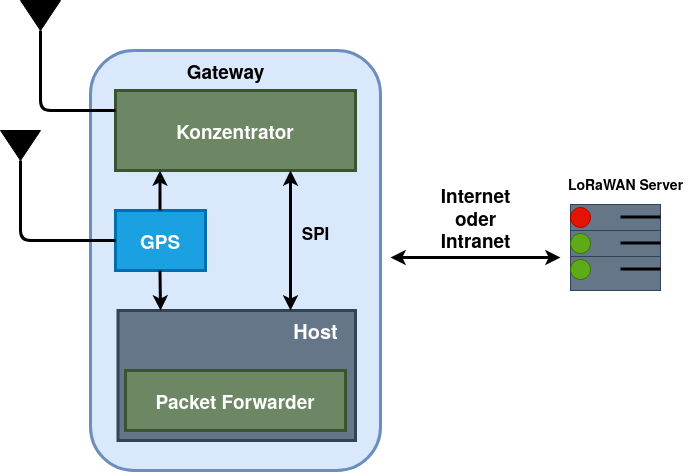
\includegraphics[ width=8cm]{source/images/LoRa_gateway}
		\label{fig:forwarder1}
	}
	\subfigure[]{
		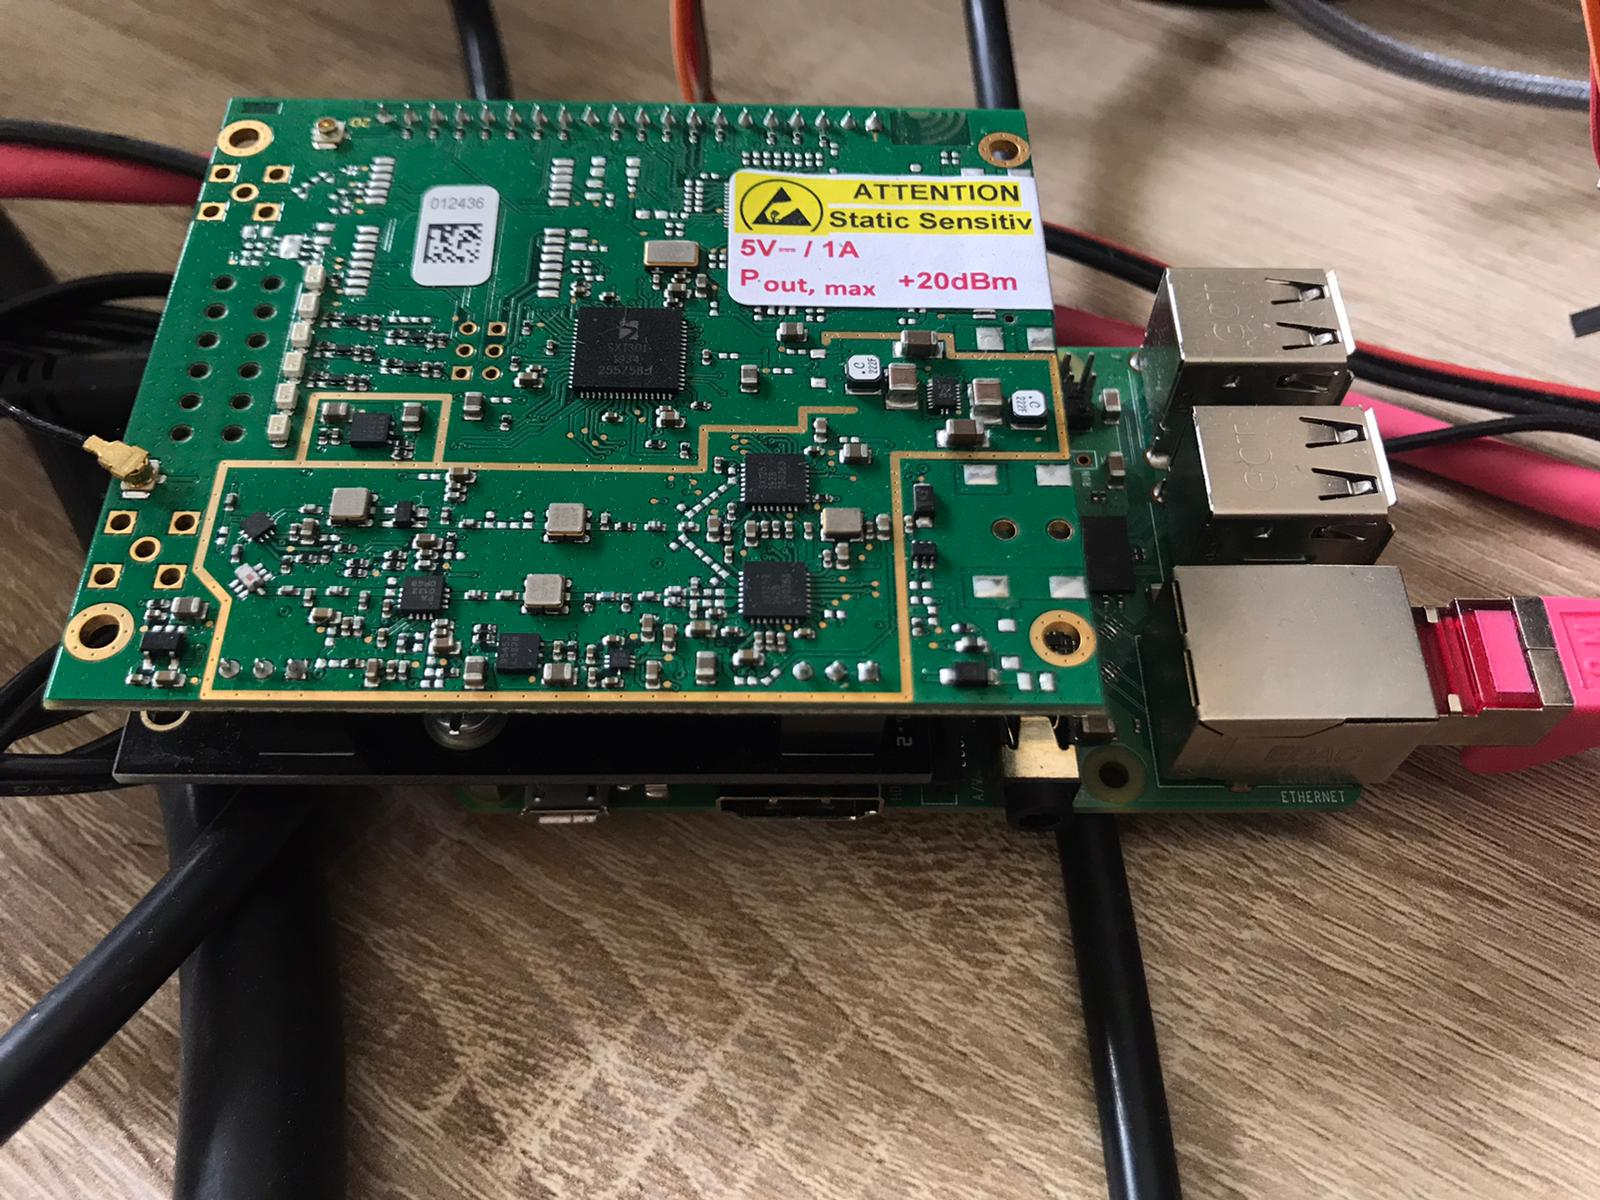
\includegraphics[width=6cm]{source/images/Gateway2}
		\label{fig:forwarder2}
	}
	\caption{LABCSMART LoRaWAN Gateway}
\end{figure}


Abbildung \ref{fig:forwarder1} zeigt die Netztwerkkomponenten, beginend mit dem Gateway und seinen Bestandteilen. Es ist deutlich zu sehen, dass das der Konzentrator und der Host durch einer SPI-Snittstelle verbunden sind und die Verbindung zwischen dem Gateway und dem Server das Internet oder Intranet ist. Unser Prototyp \ref{fig:forwarder2} ist alles in einem einzigen Modul. Das heisst, der Konzentrator, das Gateway und der Server zusammen in einem Block eingebaut sind. Der Raspberry-Pi ist gleichzeitig der Host und der Server. \textbf{(Referenzen zur Installation des Paket-forwarder im Ausblick)}

\vspace{8cm}
\section{Einstellung des LoRaWAN-Servers}\label{server}

An dieser Stelle ist die Arbeit fast fertig, da unsere Anwendung theoretisch in der Lage ist, Uplinks an dem Gateway zu schicken. Nun interessieren wir uns auf die Verarbeitung der empfangenen Daten. Die Daten werden zwar in die Luft gesendet, aber der Benutzer kann diese nicht sehen oder vearbeiten, dazu ist ein Server. Dieser Server soll in der Lage sein, gesendete Funkpakete zu interpretieren und darzustellen, sodass der Benutzer diese lesen und verstehen kann. 

Der verwendete Server heisst \textbf{lorawan-server} (Open-source). Er wurde von Herrn \textbf{Petr Gotthard} \cite{server} entwickelt und ist ein Kompater Server f"ur private LoRaWAN-Netzwerke. Dieser Server dient nicht nur als Netzwerkserver, sondern auch als Anwendungssever. Man kann damit alle Ereignisse, und alle Daten, die entweder vom Endger"at oder vom Packet-Forwarder komment. Der Server wurde in 79\% in der Programmierspache Erlang \cite{erlang} geschireben.   

In diesem Kapitel, erfahren Sie wie dieser Server einzustellen ist, um Endger"ate mit OTAA oder ABP zu verbinden. Bevor ein Endger"at hinzugef"ugt wird, muss der Server dazu vorbereitet werden. Er muss die MAC-Adresse des Gateways, der Netzwerk, das Profil des Netzwerks und die Gruppe des Endger"ats kennen. 

\begin{description}
	\item[Gateway:] Der Server kann mit einem oder mehrere Gateway verbunden werden (Nur ein in unserem Fall). Der Server bekommt alle Uplinks, die von den Gateways weitergeleitet werden,betrachtet nicht welches Endger"at welchem Netzwerk geh"ort.
	
	\begin{figure}[h]
		\centering
		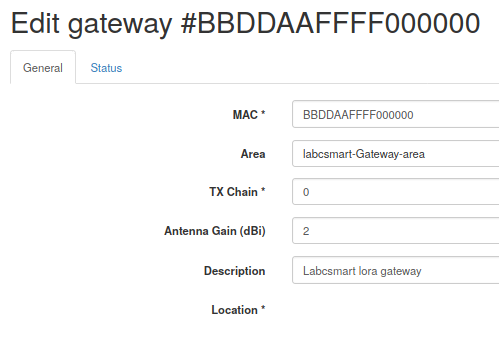
\includegraphics[width=10cm]{source/images/Gateway}
		\caption{Einstellung des Gateways\label{fig:gateway}}
	\end{figure}

	\item[Netzwerk:] Der Server kann ein oder mehrere Netzwerke verarbeiten. Jede Netzwerkkonfiguration umfasst:
	\begin{itemize}
		\item Eine Netzwerkkennung, um die Eger"at-Adresse (DevAddr) neu verbundener Endger"ate zu Erstellen.
		\item LoRaWAN-Regionparameter, einschlie\ss{}lich zus"atzliche Frequenzen
	\end{itemize}

	\begin{figure}[h!]
		% first include \usepackage{subfigure}
		\centering
		\subfigure[]{
			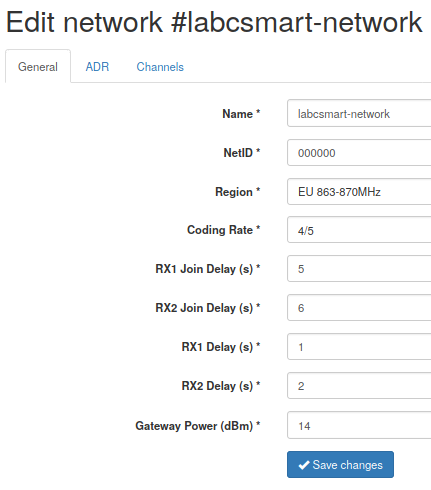
\includegraphics[ width=7cm]{source/images/Labcsmart_network_gen}
			\label{fig:NetGen}
		}
		\subfigure[]{
			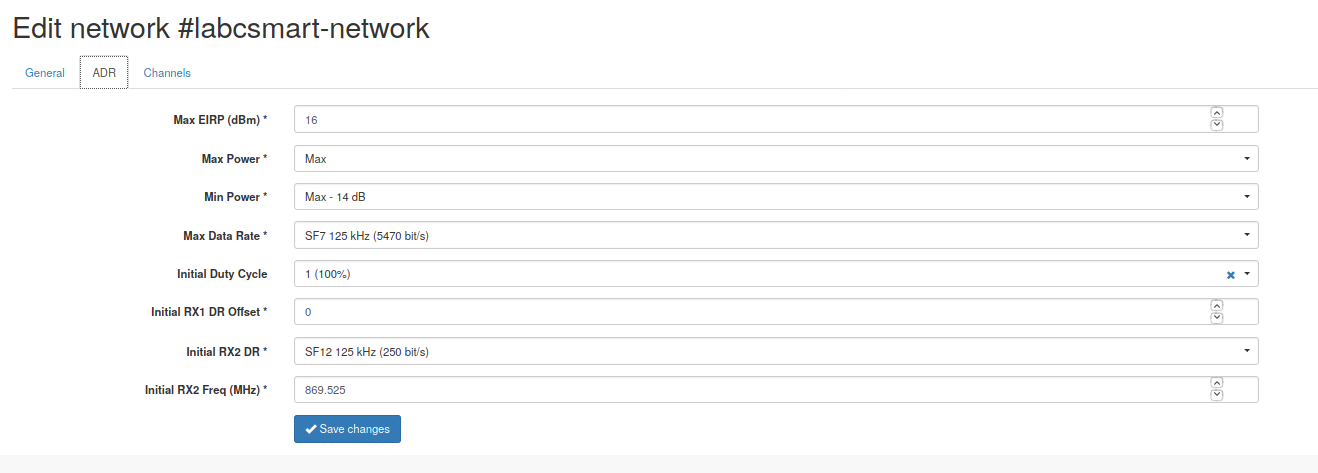
\includegraphics[width=7cm]{source/images/Labcsmart_network_adr}
			\label{fig:NetAdr}
		}
		\caption{Einstellung des Netzwerks}
	\end{figure}

	\item[Profil:] Das Profil repr"asentiert eine bestimmte Hardware und alle statischen Einstellungen in der Firmware, die f"ur eine Gruppe von Ger"aten gleich sind. Die Konfiguration umfasst:
	\begin{itemize}
		\item Die Referenz zu einem bestimmten Netzwerk
		\item Die F"ahigkei des Ger"ats, ADR (Adaptive Data Rate) durchzuf"uren oder den Batteriestatus bereitzustellen.
		\item Die Anwendung
	\end{itemize} 
	Es is zu bemerken, dass die einstellung der Abbildung \ref{fig:ProAdr} genau ist, wie die Einstellung des endger"ats, die im Abschnitt \ref{LoRaconf} erl"autert wurde. Weil wir genau dieses Ger"at im Netzwerk integrieren wollen, muss auch der Server dementsprechen eingestellt werden.

	\begin{figure}[h!]
		% first include \usepackage{subfigure}
		\centering
		\subfigure[]{
			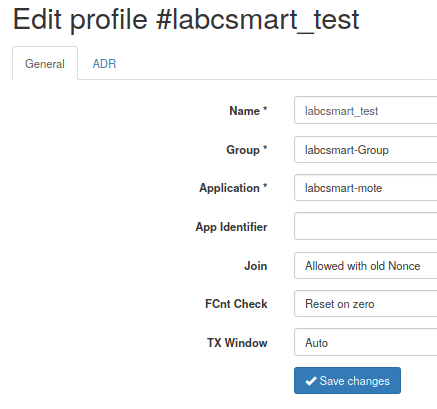
\includegraphics[ width=7cm]{source/images/Labcsmart_profile_gen}
			\label{fig:ProGen}
		}
		\subfigure[]{
			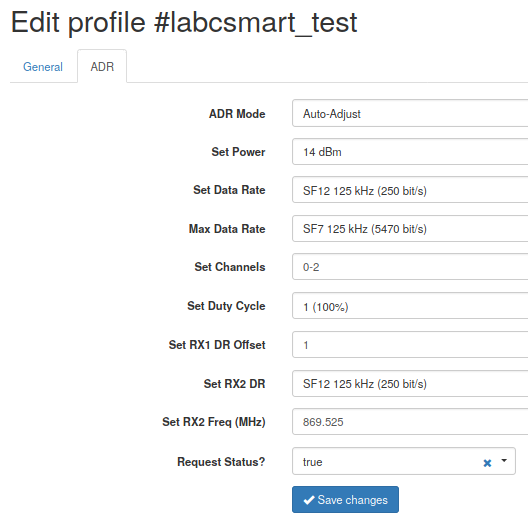
\includegraphics[width=7cm]{source/images/Labcsmart_profile_adr}
			\label{fig:ProAdr}
		}
		\caption{Einstellung des Profils}
	\end{figure}
	\vspace{10cm}
	\item[Gruppe:] Die Gruppe repr"asentiert eine Reihe von Profilen, die zu einem einzelnen Teilnetzwerk geh"oren. Zu einem einzelnen Kunde zum Beispiel.
	\begin{figure}[h]
		\centering
		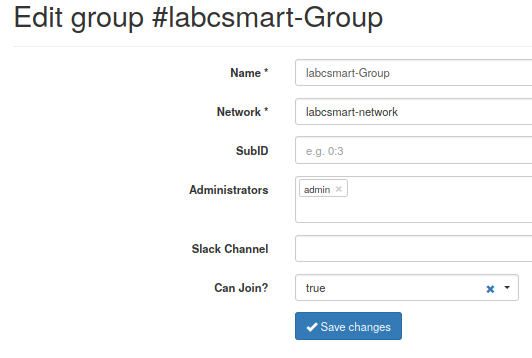
\includegraphics[width=10cm]{source/images/Labcsmart_group}
		\caption{Einstellung der Gruppe\label{fig:group}}
	\end{figure}
\end{description}

Nun ist es m"oglich Endger"ate zum Server hinzuzuf"ugen. Als erstes versuchen wir mit ABP, dann mit OTAA.
\vspace{10cm}
\subsubsection{ABP Verbindung}
Ger"ate die mit ABP verbunden werden sollen, brauchen wie im Abschnitt \ref{secure} DevAddr, NwkSKey und AppSKey.
Die Informationen auf Abbildung \ref{fig:DevAdr} werden automatisch erstellt, nachdem ein Endger"at dem Netzwerk hinzugef"ugt wurde. Man kann die "Ubertragungsfrequenzen, die Leistung und andere Einstellungen erkennen, die im Abscnhitt \ref{secure} erw"ahnt wurden. 
	\begin{figure}[h!]
	% first include \usepackage{subfigure}
	\centering
	\subfigure[]{
		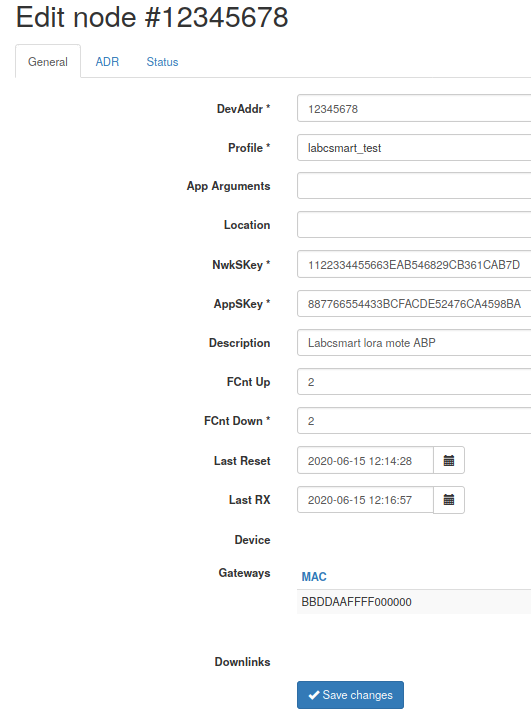
\includegraphics[ width=7cm]{source/images/Labcsmart_abp_gen}
		\label{fig:DevGen}
	}
	\subfigure[]{
		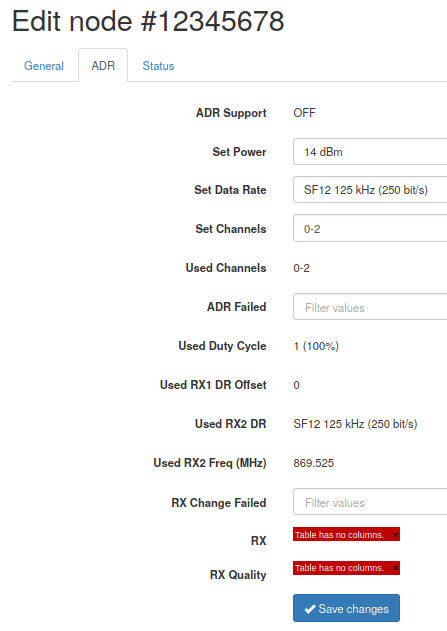
\includegraphics[width=7cm]{source/images/Labcsmart_abp_adr}
		\label{fig:DevAdr}
	}
	\caption{ABP Verbindung}
	\end{figure}

\subsubsection{OTAA Verbindung}
Hier befinden sich Ger"ate, die dem LoRaWAN-Netzwerk mit Hilfe von OTAA beitreten d"urfen. Man muss dazu aber die DevEUI, AppEUI und AppKey auf jedem Fall kennen und im Server eingeben (Siehe \ref{fig:otaa}). 
	\begin{figure}[h]
	\centering
	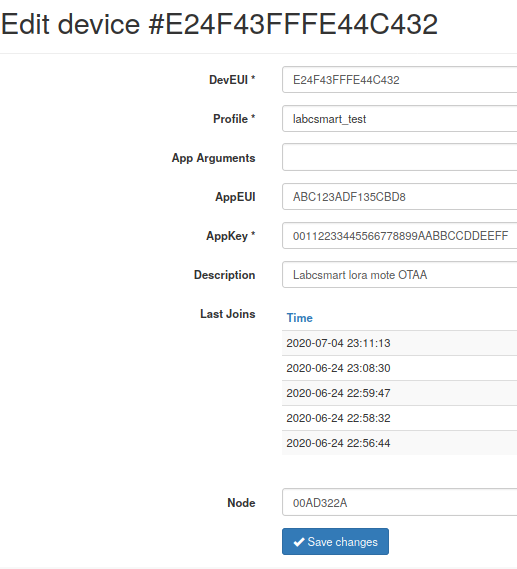
\includegraphics[width=10cm]{source/images/Labcsmart_otaa_gen}
	\caption{Einstellung OTAA\label{fig:otaa}}
\end{figure}
Nachdem das Ger"at dem Netzwerk beigetreten ist, bekommt es eine DevAddr, einen NwkSKey und einen AppSKey, die mit Hilfe des AppKey berechnet wird (Siehe \ref{secure} f"ur die Erkl"arung). 
\vspace{10cm}

Nach dem diese Einstellungen fertig sind und die Ger"ate dem Netzwerk beigetreten sind, k"onnen Uplinks im Dashboard gesehen werden. Der Inhalt (In Hexadezimal) befinden sich unter Frames (unten links vom Server). 

	\begin{figure}[h!]
	% first include \usepackage{subfigure}
	
	\subfigure[]{
		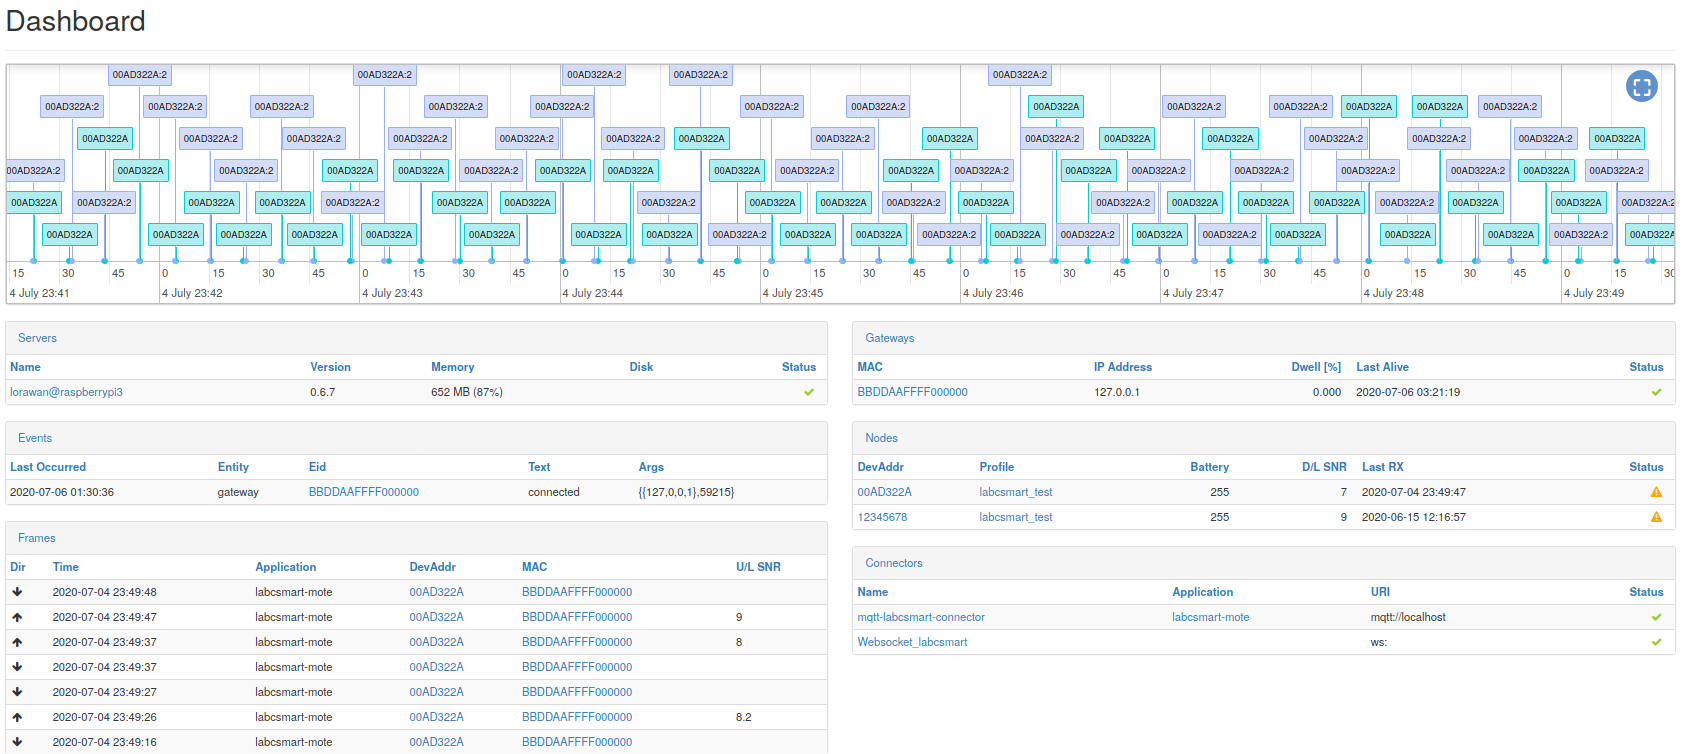
\includegraphics[ width=17cm]{source/images/dashboard}
		\label{fig:Dashboard}
	}
	\subfigure[]{
		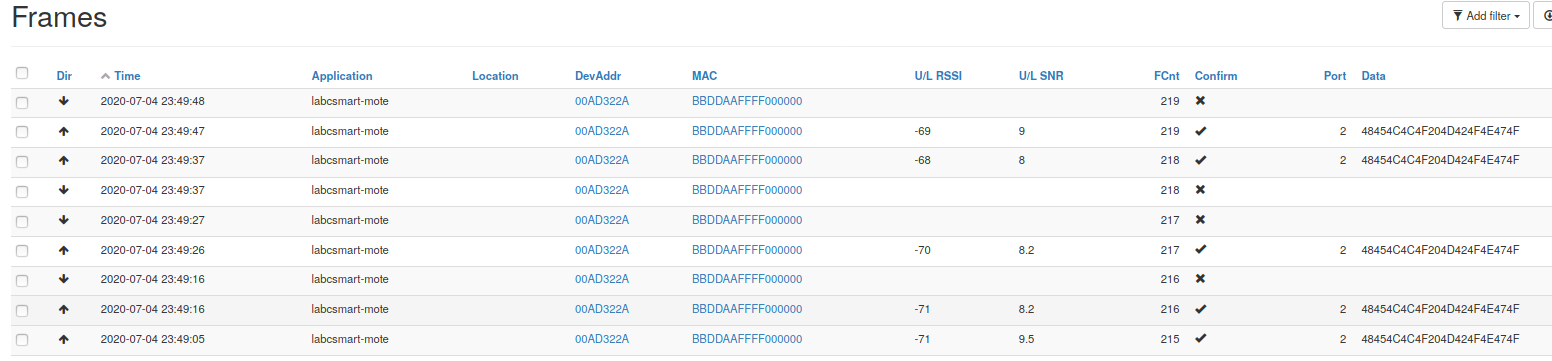
\includegraphics[width=17cm]{source/images/frames}
		\label{fig:Frames}
	}
	\caption{Zwischenergebnis}
\end{figure}
Gr"une Ereignisse im Abbildung \ref{fig:Dashboard} bezeichnen Downlinks, w"ahrend Ereignisse in lila sind Uplinks. Die Spalte U/l RSSI des Abbildungs \ref{fig:Frames} stellt die empfangene Signalat"arke (in Englisch \textbf{\textit{Received Signal Strength Indication}}, Kurzform \textbf{RSSI}) dar. RSSI ist die empfangene Leistung in miliwatts, wird aber in dBm(liste der Abk"urzung decibel miliwatt) gemessen. Diesen wird sagt wie, gut ein Empf"anger gesendete Signale empfangen kann.RSSI ist ein negativer Wert, je n"aher 0 dieser Wert ist, desto besser is das Signal. Der minimale RSSI-Wert f"ur die LoRa-Technologie ist -120dBm.  

\vspace{10cm}

Zu Ende reicht diese Ergebnis noch nicht. Was passiert wenn der Server nicht mehr funktioniert? Soll die Anwendung auch nicht funktionieren oder gibt es eine andere M"oglichkeit die Daten irgendwie zu sichern, falls ein Serverausfall vorkommen w"urde? Zwischen dem Server und dem Packet-Forwarder gibt es ein Kommunikationsprotokol Namens MQTT. Das n"achste Kapitel erkl"art was MQTT ist, wie es funktioniert und wie die Daten beim Serverausfall anderswo gesichert werden k"onnen. 

\vspace{10cm}   
\section{MQTT brocker zur Daten"ubertragung}


\chapter{Software-Entwicklung}\label{Soft-Ent}
\section{Entwicklungsumgebung}
\subsection{Eclipse}
\subsection{Libopencm3 Bibliotek installieren}
\section{Sensoren Auslesen} \label{Sensoren}
\section{LoRa Commandos senden}
